% The document class supplies options to control rendering of some standard
% features in the result.  The goal is for uniform style, so some attention 
% to detail is *vital* with all fields.  Each field (i.e., text inside the
% curly braces below, so the MEng text inside {MEng} for instance) should 
% take into account the following:
%
% - author name       should be formatted as "FirstName LastName"
%   (not "Initial LastName" for example),
% - supervisor name   should be formatted as "Title FirstName LastName"
%   (where Title is "Dr." or "Prof." for example),
% - degree programme  should be "BSc", "MEng", "MSci", "MSc" or "PhD",
% - dissertation title should be correctly capitalised (plus you can have
%   an optional sub-title if appropriate, or leave this field blank),
% - dissertation type should be formatted as one of the following:
%   * for the MEng degree programme either "enterprise" or "research" to
%     reflect the stream,
%   * for the MSc  degree programme "$X/Y/Z$" for a project deemed to be
%     X%, Y% and Z% of type I, II and III.
% - year              should be formatted as a 4-digit year of submission
%   (so 2014 rather than the academic year, say 2013/14 say).

\documentclass[oneside,% the name of the author
                    author={Malak Hajji},
                % the degree programme: BSc, MEng, MSci or MSc.
                    degree={BSc},
                % the dissertation    title (which cannot be blank)
                    title={Designing An Accessible Computational Toolkit For Students},
                % the dissertation subtitle (which can    be blank)
                  subtitle={With Mixed Visual Abilities}]{dissertation}
\usepackage{float}

\usepackage{multirow}
\usepackage{subcaption}
\usepackage{placeins}
\begin{document}

% =============================================================================

% This section simply introduces the structural guidelines.  It can clearly
% be deleted (or commented out) if you use the file as a template for your
% own dissertation: everything following it is in the correct order to use 
% as is.

% =============================================================================

% This macro creates the standard UoB title page by using information drawn
% from the document class (meaning it is vital you select the correct degree 
% title and so on).

\maketitle

% After the title page (which is a special case in that it is not numbered)
% comes the front matter or preliminaries; this macro signals the start of
% such content, meaning the pages are numbered with Roman numerals.

\frontmatter


%\lstlistoflistings

% The following sections are part of the front matter, but are not generated
% automatically by LaTeX; the use of \chapter* means they are not numbered.

% -----------------------------------------------------------------------------

\chapter*{Abstract}

\vspace{1cm} 

\noindent
Programming is becoming a fundamental skill, and incorporating computational thinking (CT) into early childhood education is now widely recognised as being extremely beneficial for a variety of reasons. CT's value extends beyond computing contexts, with the potential to influence children's social, emotional, and cognitive development, as well as their personal and professional development. However, many computational environments aimed at promoting early learning of basic computational concepts and practises, are inaccessible to learners with visual impairments. These impediments begin  with visual tools and visually demanding outputs that are often not compatible with accessible technology such as screen readers. Previous approaches aimed to bridge this gap by using tangibles to program, however they are often expensive systems and the output usually consists of audio stories or music. During this project, I aimed to develop an inexpensive system that allows young students to learn to program robots, specifically the Ozobot, using a tangible block-based user interface.  The system was developed through two design consultations with experts and potential users. The system was also evaluated with user testing and surveys to determine its usability and level of engagement. The general consensus was that the system was effective for teaching basic computational thinking skills and programming concepts. Future iterations of my system will focus on maximising the opportunities for accessible and enjoyable learning experiences by extending the system to include more complex programming concepts, such as conditional statements and a game for the Ozobot robot to complete.


% -----------------------------------------------------------------------------


\chapter*{Dedication and Acknowledgements}

{\bf A compulsory section}
\vspace{1cm} 

\noindent
It is common practice (although totally optional) to acknowledge any
third-party advice, contribution or influence you have found useful
during your work.  Examples include support from friends or family, 
the input of your Supervisor and/or Advisor, external organisations 
or persons who  have supplied resources of some kind (e.g., funding, 
advice or time), and so on.

% =============================================================================

% After the front matter comes a number of chapters; under each chapter,
% sections, subsections and even subsubsections are permissible.  The
% pages in this part are numbered with Arabic numerals.  Note that:
%
% - A reference point can be marked using \label{XXX}, and then later
%   referred to via \ref{XXX}; for example Chapter\ref{chap:context}.
% - The chapters are presented here in one file; this can become hard
%   to manage.  An alternative is to save the content in seprate files
%   the use \input{XXX} to import it, which acts like the #include
%   directive in C.


% -----------------------------------------------------------------------------


\chapter*{COVID-19 Statement}

{\bf An optional section, of at most 800 words} 
\vspace{1cm} 

\noindent
A summary of any planned research activities disrupted by Covid-19 restrictions and the extent to which it was possible to adapt the work in those changed circumstances. If the project was able to go forward as planned, you can safely remove this section without losing any marks. The following may be included:

\begin{itemize}
\item Details of any planned research activities curtailed by the pandemic because of, for example, lack of access to facilities, libraries, archives, research participants, fieldwork, etc. Information on any curtailed training should be included only insofar as it relates to the impact on research activities and on the dissertation.

\item An acknowledgement of the anticipated contribution and value to the dissertation if those research activities had not been curtailed and what was possible to include in the dissertation in the circumstances, including where alternative choices were made to adapt the work and whether there are any weaknesses that could not be overcome.

\item Any other relevant factors on the impact of Covid-19 on research activities and on the contents of the dissertation.

\item Details of any research activities required by the examiners as part of a resubmission that were curtailed by the pandemic may be included in a new or revised Covid-19 statement in the resubmitted dissertation.
\end{itemize}

% -----------------------------------------------------------------------------

% This macro creates the standard UoB declaration; on the printed hard-copy,
% this must be physically signed by the author in the space indicated.

\makedecl



% -----------------------------------------------------------------------------

% LaTeX automatically generates a table of contents, plus associated lists 
% of figures and tables.  These are all compulsory parts of the dissertation.

\tableofcontents
\listoffigures
\listoftables

% -----------------------------------------------------------------------------



\chapter*{Ethics Statement}

{\bf A compulsory section} 
\vspace{1cm} 

In almost every project, this will be one of the following statements:
    \begin{itemize}
        \item ``This project did not require ethical review, as determined by my supervisor, [fill in name]''; or
        \item ``This project fits within the scope of ethics application 0026, as reviewed by my supervisor, [fill in name]''; or
        \item ``An ethics application for this project was reviewed and approved by the faculty research ethics committee as application [fill in number]''.
    \end{itemize}
    
See Section 3.2 of the unit Handbook for more information. If something went wrong and none of those three statements apply, then you should instead explain what happened.


% -----------------------------------------------------------------------------



% -----------------------------------------------------------------------------



% -----------------------------------------------------------------------------

\chapter*{Notation and Acronyms}

{\bf An optional section}
\vspace{1cm} 

\noindent
Any well written document will introduce notation and acronyms before
their use, {\em even if} they are standard in some way: this ensures 
any reader can understand the resulting self-contained content.  

Said introduction can exist within the dissertation itself, wherever 
that is appropriate.  For an acronym, this is typically achieved at 
the first point of use via ``Advanced Encryption Standard (AES)'' or 
similar, noting the capitalisation of relevant letters.  However, it 
can be useful to include an additional, dedicated list at the start 
of the dissertation; the advantage of doing so is that you cannot 
mistakenly use an acronym before defining it.  A limited example is 
as follows:

\begin{quote}
\noindent
\begin{tabular}{lcl}
AES                 &:     & Advanced Encryption Standard                                         \\
DES                 &:     & Data Encryption Standard                                             \\
                    &\vdots&                                                                      \\
${\mathcal H}( x )$ &:     & the Hamming weight of $x$                                            \\
${\mathbb  F}_q$    &:     & a finite field with $q$ elements                                     \\
$x_i$               &:     & the $i$-th bit of some binary sequence $x$, st. $x_i \in \{ 0, 1 \}$ \\
\end{tabular}
\end{quote}

% -----------------------------------------------------------------------------

\mainmatter

\chapter{Introduction}
\label{chap:introduction}
\section{Motivation}
Computing education for all young children is now widely recognised as being extremely beneficial for a variety of reasons. Learning to code teaches children not only how to program and interact with computers, but also how to solve problems using logical and creative thinking \cite{CB-intro1}, also known as 'computational thinking'. Computational Thinking (CT), like reading and writing, is becoming a fundamental literacy skill. CT's value extends beyond teaching computing concepts, with implications for children's social, emotional, and cognitive development\cite{intro,cognition-intro}, as well as personal and professional development\cite{CB-CT1}. 

Although there is no one-size-fits-all approach to teaching computational thinking to young children, most research scenarios include visual block-based programming languages with graphical outputs, such as Scratch\cite{scratch} and Blockly\cite{blockly}. Because these platforms are block-based, the children can tinker with the various digital blocks and put together sequences of instructions rather than having to learn how to read the syntax of traditional programming languages. They are actively involved in the development process while also developing their own ideas, which piques their interest in learning how to implement new functionalities using new computational concepts.

Physical artefacts, such as robotic kits and toys, are also used to teach CT to young children, allowing them to actively engage with their environment and learn through interactive play, without using screen-readers, a keyboard, or a mouse. Robots immerse children in a playful learning environment, promoting the development of computational thinking skills, such as problem-solving and thinking at various levels of abstraction. Children are better prepared for future programming tasks and also develop their spatial cognition development\cite{intro-robots}.

\section{Problem}
Engaging in computing from a young age can be difficult for visually impaired (VI) children, as many computing curricula use Graphical User Interfaces (GUI) to teach CT. These tools are inaccessible to VI students as their outputs are usually visual (e.g. Scratch), they are often incompatible with screen readers and their syntax is hard to understand via audio output.

Previous research efforts to make CT accessible to VI children have been largely limited to audio-based actions, preventing VI children from participating in spatial programming activities like their sighted peers, and thus isolating them in the classroom. Previous approaches, such as Storyblocks\cite{storyblocks} and Project Torino\cite{torino} , use tangibles to make programming accessible to all. However, the output of their activities consists of audio stories or music  which is unsuitable for hearing impaired students.
Furthermore, Torino is expensive to purchase and StoryBlocks has not been developed past the research stage or properly tested yet, like many other systems. 
I sought to bridge this gap and develop a fully tangible solution accessible to children with mixed visual abilities.
\section{Approach}
In this dissertation, I propose the implementation of a tangible user interface (TUI). The TUI is composed of tangible blocks that construct computer programs and a robotic device, the Ozobot, to produce an accessible multimodal output, while engaging children with mixed visual abilities in learning computational thinking. 

The execution of this project followed an iterative design process. I started by conducting a literature review on the existing programming languages and toolkits to understand the qualities and flaws present in current programming environments for children. I then created an initial block prototype based on my findings. Following this, I conducted interviews with Special Needs Educators (SNEs) to determine what makes a TUI accessible to mixed visual abilities. I then ran a design workshop with a group of students, where I presented different design prototypes of my tangible blocks. The participants interacted with each design and gave feedback, to ensure the final implemented design is intuitive and engaging.

After the design studies, I considered the results and created a final fully tangible system. The proposed solution is composed of tangible blocks with embossed icons to represent actions, magnets to facilitate block coupling and ArUco markers to allow for block detection. The blocks are colored with high contrast colors to be accessible to low vision users too.
The technical aspect of the system detects the Aruco markers present in the  workspace and translates them to actions for the Ozobot robot to execute. 
At the end of my project, I conducted user testing sessions to evaluate my system and identify aspects that could be improved in the future. After that, I summarise my findings from this project and discuss future work that could optimise the usability and functionality of my system.

\section{Aims and Objectives}

\begin{quote}
\noindent
The high-level objective of this project is to create a tangible, accessible coding platform for students with mixed visual abilities. More specifically, the concrete aims are:

\begin{enumerate}
\item Research literature and current approaches to teaching computing to students both sighted and visually impaired.
\item Examine how current tangible tools for teaching computational thinking in the classroom can be adapted for use by students with visual impairments.
\item Adopt a co-design approach with experts and conduct a design workshop with users to decide on the overall design of the system.
\item Create universal, tactile symbols that describe robot actions and can be understood by the majority of students.
\item Implement a fully tangible system, composed by tangible blocks, the Ozobot and a software that connects the two.
\item Perform user testing to ensure the system is engaging and can effectively teach basic coding skills.
\end{enumerate}
\end{quote}


% -----------------------------------------------------------------------------

\chapter{Contextual Background}
\label{chap:context}

\section{Introduction}

Computer science and programming have become extremely useful in everyday life, and incorporating computing into the education of all young children has become critical for a variety of reasons. Learning to program allows young students to actively engage with computers while also teaching them how to deconstruct, analyse, and solve problems in a logical and creative manner \cite{CB-intro1}.
Additionally, previous research has found that it is critical for children to begin computing education as early as possible, because stereotypes about who can and cannot code are formed at a young age \cite{CB-intro2, CB-intro3}.
Computing concepts are first introduced in primary school as computational thinking skills. By learning computational thinking at a young age, children are better prepared to assimilate programming languages later on in their education. 
In this section, I will discuss the motivations behind computational thinking learning and give an overview of current computational tools used to teach CT in UK schools. I will then explore how computing is taught to learners with mixed visual abilities, as well as the challenges they face and analyse the different inclusive computational tools and their limitations. By combining the background on computational thinking learning and current limitations with  inclusive environments, I aim to design a fully accessible tangible  and robotic coding environment for mixed visual abilities.

\section{Learning Computational Thinking}  
\subsection{Motivations for Computational Thinking}
Computational thinking is becoming a fundamental skill for everyone, not just computer scientists, and just like reading, writing and arithmetic, computational thinking should be a part of every child’s analytical ability. It is defined as “the thought process involved in formulating a problem and expressing it in a way that a computer –human or machine- can effectively carry out.” \cite{CB-CT1}. CT draws on the concepts fundamental to computer science, such as sequences and operators as well as practices like logical reasoning, testing, debugging and abstraction. The value of CT does not just lie in computing, it can be used to support problem solving across all disciplines, including the humanities, math and science. Therefore, acquiring CT as a skill impacts the social, emotional and cognitive development of children, while encouraging personal and career growth.


\subsubsection{Low floor, high ceiling and wide walls}

Brennan and Resnick \cite{resnick11} developed a framework for computing education that includes seven computational concepts (sequence, loops, events, parallelism, conditionals, operators, and data) and four computational practises (experimenting and iteration, testing and debugging, reusing and remixing, abstracting and modularizing). Since CT learning has become widely spread, it prompted researchers and designers to develop an abundance of new toolkits and computing environments to teach some of these concepts in a way that is enjoyable and accessible to increasingly younger learners. The idea of “low floor, high ceiling and wide walls” is one of the guiding principles for the creation of these environments for children \cite{CB-lowfloor}. It essentially means that it should be easy for a beginner to cross the threshold to create working programs (low floor) and the tool should be extensive enough to satisfy the needs of advanced programmers (high ceiling). Wide walls have been described as one of the most crucial features for computational thinking tools as they enable diverse exploration and encourage creativity \cite{CB-lowfloor}. Computational toolkits have been widening the walls by increasing the number and type of outputs supported and by enabling children to move beyond a specific set of “recommended activities”. 

Several programming tools used to teach computational thinking fit these criteria to varying degrees. Some of the most widely used graphical programming environments in education are Scratch\cite{scratch}, Blockly \cite{blockly}; and robotics kits and tangible media such as Arduino and BeeBot. These tools are very efficient in learning computational thinking because they are relatively easy to use and allow young students to focus on designing and creating, while avoiding issues of programming syntax, fitting the 'low floor' principle. Tangible user interfaces (TUIs) are another common strategy for assisting children in learning basic computational concepts by providing children with physical objects to think with and allowing them to use their bodies. Other graphical user interfaces (GUI) have also been widening the walls by expanding the  types of outputs supported, to include visual outputs such as moving animations, blinking LEDs, or sound outputs \cite{lee}, to create multisensory effects\cite{multisensory,scratch}. Finally, many computational toolkits place a strong emphasis on haptic outputs, particularly through the use of robots that can move around in space in response to specific commands such as The Lego Mindstorms Kit \cite{lego-mindstorm}.

To summarise, several of the tools used to teach young children are guided by the principle of 'low floor, high ceiling, and wide walls,' and they have proven to be extremely effective in introducing computational thinking skills. As my project is aimed at the same age group, I will design my system around the aforementioned principle, with the goal of creating a tangible programming interface with a low programming threshold that also allows for improvement and encourages diverse exploration and creativity for people of mixed visual abilities.

\subsection{Computational Thinking in UK Schools}
As I aim to create a system to support young children in learning computational thinking, it is important to gain an insight about the current computing curricula.
The UK curriculum provides a concrete example of the adaptation of computational thinking learning in early childhood. When computing was added to the national curriculum in England in 2014, it became mandatory for primary school children to learn computational thinking skills starting at the age of five \cite{education-department}.
The introduction of computational thinking to children at a young age has proven to be very beneficial, as it has established early confidence in technology, which can help encourage children to pursue Computer Science in higher education\cite{confidence}.

In Key Stage 1, computational thinking skills are developed through the use of floor robots such as the BeeBot and the LOGO turtle. Learners are expected to figure out what each floor robot command does and then use that information to create an algorithm to move their robot around the mat. \cite{robot-KS1,education-department,curricula}. As a result, students are exposed to the early stages of program design using algorithms, which is a form of computational thinking. This is accomplished by learners outlining their task by identifying the robot's route's beginning and ending points. This outlining will ensure that learners have a clear understanding of what they want to accomplish with their program\cite{curricula}.

Students in Key Stage 2 are introduced to visual programming languages like Scratch\cite{scratch}, which allow them to experiment with more complicated programming concepts like loops and conditional expressions. Visual languages are commonly used at this age because they allow pupils to code without having to learn complex syntax \cite{curricula}. Furthermore, visual languages are most adapted to their cognitive development at this age\cite{cognitive}. The concepts taught in visual languages are easily transferable to text-based languages, and they provide a foundation of skills that may be built upon.

\section{Visual Programming Languages}

In this section, I will discuss the motivations behind the learning of computational thinking through the use of visual programming environments and languages in primary schools.
I will then discuss the limitations in these environments, particularly for students with visual impairments, to design a suitable alternative.

\subsection{Types of Languages and Benefits}
\subsubsection{Block-based languages}
\begin{figure}
    \centering
    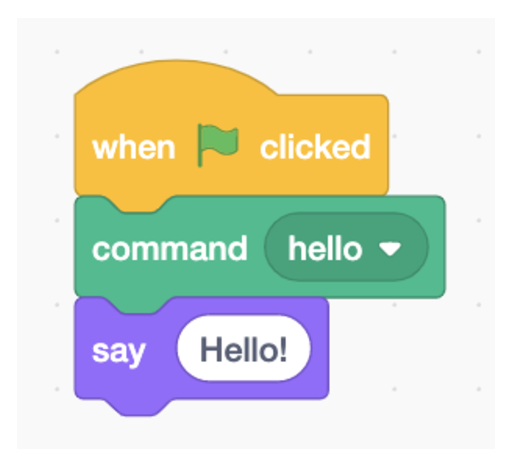
\includegraphics[width=0.3\textwidth]{thesis/scratch.eps}
    \caption{Block-based Programming Language Scratch ~\cite{scratch}}
    \label{fig-scratch}
\end{figure}
Computer programming can be a way of teaching computational thinking and most research scenarios consider block-based programming languages with graphical outputs, such as Scratch\cite{scratch}, a direct and defined strategy to teach young children computational concepts\cite{blocks}. These platforms often introduce many programming activities that can be personalized and to the user's interests, which can keep children engaged and motivated to build their own projects. Children can also tinker with the different digital blocks and put together sequences of instructions, as opposed of having to learn how to read the syntax from traditional visual programming languages. This allows young students to build their own ideas and gain confidence in their novice programming skills while growing an interest in learning new more complex computational concepts.\cite{confidence}


\subsubsection{Block and Icon based languages}
Previous research has shown that students as young as four years old can understand basic computer programming concepts and build and program robotics projects\cite{bers}. However, it is hard for illiterate children to understand blocks with written statements such as the blocks in Scratch. Thus, icons in block programming have been widely used to introduce computing concepts to younger demographics. Children can easily recognise icons because they relate to everyday activities and make the interface more understandable. 
An example of such a platform is ScratchJr\cite{scratchjr}, the redesign of the Scratch platform for the developmental and learning needs of children from kindergarten to second grade. Children can put together blocks identified with icons to form instructions and have a graphical output, thus eliminating the need to read blocks while maintaining the user engaged.

\subsubsection{Text-based languages}

Text-based languages are less utilised to teach younger children computational thinking as it requires the children to be familiar with the syntax. It is important to note that the UK primary computing curriculum is not about teaching children a specific programming language, rather than understanding the principals of programming and applying these to solve specific problems.\cite{curricula} Thus, unlike KS3, where the national curriculum states that students should use a text based programming language, this is not a requirement in primary schools, and generally block-based programming environments are used.

\subsubsection{Impact on Future Education }
Several studies have been carried out to investigate the transition from block-based and graphical languages used in primary schools to text-based languages later in education. Students who took Scratch programming classes in middle school were tested to see if they performed better in a high school text-based programming course\cite{phd}. Scratch students outperformed their peers in some areas, according to the researchers. For example, they had a much better grasp and understanding of computational concepts like looping. The authors also discovered qualitative differences between the two groups, with students who had previously used Scratch reporting higher levels of self efficacy and motivation to learn to code.

Another study\cite{study2-impact} demonstrated that a blended approach between block-based and text-based languages enables students to better understand the high-level programming concepts rather than focus on the low-level compilation errors. Students were more confident using the text-based environment after gaining familiarity with the block-based language. 
 
\subsection{Limitations}

Visual Programming Languages (VPL) used in primary schools are inaccessible to visually impaired and motorically challenged individuals\cite{motorical}. Although they  allow users to easily create programs by arranging graphical blocks logically, visual languages are completely dependent on the use of a mouse and keyboard, which makes it impossible for students with a mobility impairment to use them independently. Due to the drag-and-drop nature of assembling code in most systems, visually impaired students may find it difficult to assemble program, especially if they are unable to track the mouse on the screen. Furthermore, the vast majority of VPLs are inaccessible to screen readers. As a result, visually impaired students must rely on a sighted peer or teaching assistant to explain programming blocks\cite{limitations}. In mainstream schools, this takes away a student's independence when coding and isolates them from their sighted peers.


\section{Computing in Special Education}
In this section, I define the scope of the project by describing how children with mixed visual abilities are taught in the UK. I then discuss existing tools for computational learning and physical computing in special educational settings, to comprehend the significance of inaccessible programming teaching methods.

\subsection{Teaching Learners with Mixed Visual Abilities}

In the UK, more than two million people are living with sight loss and approximately 25,660 of children up to the age of 16 have a vision impairment\cite{nhs,rnib}. The majority of blind and low vision children are taught in mainstream schools\cite{rnib}. The mainstreaming of learners with disabilities was driven by a vision of social inclusion supported by inclusive teaching practices\cite{parliment}. Learners are supported by qualified teachers of the visually impaired (QTVI) who help children adapt to the mainstream curriculum. There are also a very few specialist schools that work with blind and low vision students who have an additional or profound disability. This variety suggests that the mainstream national curriculum needs to work across a wide range of children abilities. 

In practise, an inclusive approach to education necessitates the use of multisensory teaching techniques to ensure that all students, regardless of their abilities, can participate. However, due to a lack of resources and time on the part of teachers, as well as new non-accessible and non-inclusive technologies in schools, implementing mainstream education for disabled children has proven to be difficult, limiting their academic and social participation.\cite{gray}. 

As a result, the emphasis has shifted to making in-class materials accessible and inclusive for all students. This has been especially difficult in STEM subjects\cite{moon}, and there have been a number of tried solutions. One suggestion, for example, was to pair disabled and non-disabled students and divide the work according to abilities. A sighted learner manipulates a programming environment like Scratch, whereas a visually impaired child suggests ideas for an animation he will never see. However, this method only allows the visually impaired pupils to partially participate, if at all. Teaching assistants (TA) are also frequently asked to fill in the gaps and make their own modifications in order to create accessible computational tools. This method frequently results in focused interactions between the TA and the student, as well as the formation of an assistance bubble that isolates disabled students from the rest of the class\cite{metatla}. As a result, there is a significant gap between the idealised social inclusion in education and the reality of computing education.

\subsection{Inclusive Computational Learning Tools}

A range of tools have been developed to support computational learning for learners with mixed visual abilities and to bridge the gap in computing in special education. Most of these tools aim to make code structures apparent in order to make existing programming languages more accessible or compatible with assistive technology such as screen readers or magnification software. In this section, I will consider both advantages and limitations of some accessible computational tools to influence my system’s design decisions. 

\subsubsection{Quorum}
Quorum \cite{quorum}is an accessible evidence-based programming language. The main aim of Quorum is to simplify syntax to provide accessibility for visually impaired students. The simplified syntax helps students better understand code as it is read aloud using screen readers or displayed on a braille device. Quorum can be an effective tool for those who already know how to code, but is less suitable for novices. Like many other text-based languages, it can be challenging to teach to younger students to use Quorum because they have to be familiar with the language syntax and keywords.

\subsubsection{JBrick}
JBrick\cite{jbrick} is a technology that simplified the browsing and entry of text commands and code compilation through visual and audio-feedback, which helps visually impaired teenagers program the Lego MindStorms robots. The system works with JAWS, the aforementioned screen reader for Windows, and ZoomText, a software for screen magnification. Thus, the JBrick environment requires students to be proficient with screen readers and is more suitable for older visually impaired students.

\subsubsection{Javaspeak}
JavaSpeak\cite{javaspeak} is an editor providing additional information about the structure and semantics of written Java code, to assist computer science majors with VI to learn how to program in Java. Similarly to JBrick\cite{jbrick}, Javaspeak  relies on screen readers to read the code structure. This system is designed for university students and is not suitable for younger children who have limited knowledge with semantics and are not fully proficient in using a screen-reader and keyboard.

\subsubsection{Blocks4All}
Blocks4All is an accessible block-based programming environment\cite{blocksforall}.The application was developed for a touchscreen Apple iPad due to the built-in screen reader VoiceOver and zoom capabilities. It features puzzle shaped blocks that fit together by the shape of the design and by the audio feedback from the app. The system is an audio-based drag and drop system, so the user receives audio feedback describing the blocks locations to help move them. The Blocks4All environment is used to control a Dash robot as an tangible output for visually impaired children. This allows students to feel and hear the output of thee programmed commands through the movement or sounds made by the Dash robot. As Blocks4All heavily relies on audio representation using VoiceOver, the system may not be suitable for children who are deaf. In addition to this, most visually impaired students prefer spatial representation to audio representation since they use a spatial mental model to remember information.

\subsubsection{StoryBlocks}
StoryBlocks\cite{storyblocks} is a tangible programming toolkit that was designed for VI users to create audio stories. The system is composed of blocks that represent story components such as characters and actions. The system captures the blocks with a camera when they are put together on the workspace and outputs a translated audio story. The blocks are all identifiable by icons with distinct shapes and colors. The shape of each block indicates how it can be connected to other blocks and is marked with a distinctive dot pattern to be recognized by the program running on the mobile device. StoryBlocks was designed as a combination of tangible programming blocks and audio output, which is a compelling way to teach basic computational concept, particularly for visually impaired individuals.

\subsubsection{Torino}
\begin{figure}
    \centering
    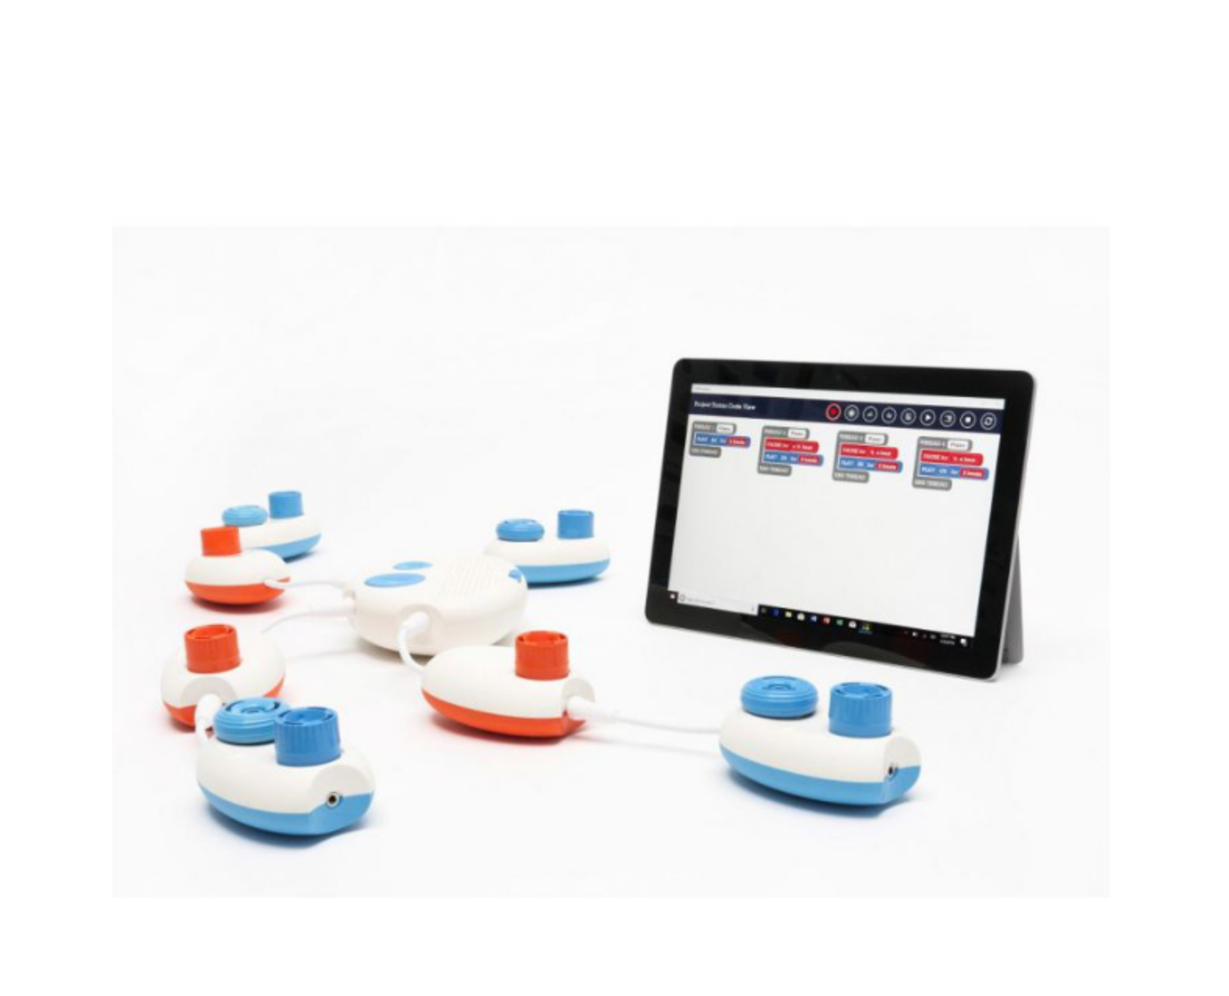
\includegraphics[width=0.5\textwidth]{thesis/torino.eps}
    \caption{Torino/Code Jumper\cite{torino}}
    \label{fig-torino}
\end{figure}
Torino\cite{torino} is a physical programming language to teach computational thinking to children between 7 and 11 years old with mixed visual abilities. It is one of the first systems made to teach basic programming to primary school students. The system is composed of plastic pods acting as instruction beads that can be physically connected and manipulated to generate sound as output. There are three types of beads: play, pause, and loop, and they each translate to a line of code in the program. Each bead further has buttons to control the repetition of the sound to be played, or to increase or decrease the length of pause and play executions, introducing the concept of variables. There is also a Code Jumper hub unit which allows the user to press play and pause on execution and read aloud the code. Students can connect pods to each other and to the hub by the use of jumper cords, creating programs with sound output. The Code Jumper app can connect to the hub unit to view the code visual format and it is also made accessible for screen readers and magnification software.  

The exploration of the beads is  critical for VI children to understand their functionalities. Thus, to facilitate their identification, each pod is distinct in size and shape, and is colored using high contrasting colors. In the end, the creators of Code Jumper were able to infer that touch, audio feedback, and visual representation are essential in the design of inclusive tools for VI children.
However, this system is unpractical for classroom use. It is composed of costly custom electronic components, and may not be within the budget of many schools. Broken equipment will also be hard and expensive to replace or repair. Since it relies on audio output, Code Jumper is also unsuitable for children who are deaf or hard of hearing as they may be unable to understand the output of the system.

\section{Summary}
Throughout this chapter, I have considered the technologies that can be used to teach computational thinking to younger students, as well as how these tools can be modified to make them accessible to people with VI. Furthermore, I investigated the accessible methods available for those with VI to learn CT and evaluated their suitability for use by younger students. The main takeaway is that existing accessible languages cannot be used with young children, as they require previous knowledge about language syntax or technologies like screen readers. Other accessible technologies, such as StoryBlocks and Torino, have either not been thoroughly tested or are prohibitively expensive. In the following section, I will present publicly available tangible systems that are similar to my proposed system. 
% -----------------------------------------------------------------------------

\chapter{Related Work}
\label{chap:related}
In this chapter, I will explore tools with similar features to the system I am building, to determine their successes and limitations. The tools studied include examples of tangible programming tools and robots used to teach computing concepts to young students. I will also make a comparison of their features and other characteristics such as output types, price, and accessibility, to draw out the limitations they could pose for visually impaired students. From this discussion, I will then aim to develop an initial set of required features to design a system that is accessible to mixed visual abilities.

\section{Tangible Tools for Learning}

Tangible Tools or Tangible User Interfaces (TUI) are an alternative to visual programming for younger learners. They are composed of physical pieces, that are often puzzle-like pieces, that are put together to generate code. Tactile tools often use icons to convey the meaning of the physical piece. This allows the tool to be universally understood and suitable for use with younger children. Tactile learning methods have been praised for their ability to aid students in understanding concepts. As young children have a deep and implicit spatial knowledge, it is more intuitive for them to grasp computational concepts by moving physical pieces to manipulate another body i.e a robot. Thus, tangible tools such as LOGO and BeeBot are widely used in KS1 and KS2 to teach computational thinking. [https://www.nfer.ac.uk/publications/FUTL69/FUTL69.pdf]
In order to identify features that make tangible tools accessible, I have explored several commercially available tangible toolkits used to teach young children computational thinking through coding.

\subsection{Examples of TUI}
\subsubsection{Osmo}
Osmo is a mobile application that utilises a mirror attached to the Apple iPad to capture tangible blocks placed on the workspace in front of the iPad. These blocks are detected by the system and used to play different games and display visual effects on the screen. Children can assemble coding blocks on the work surface to control a character on the screen on the Osmo Coding Awbie game. The blocks instruct the robot like character to traverse an environment. The output and feedback from this system is purely visual and is not compatible with screen readers. Additionally, the blocks themselves only show visual information and do not have embossing for a tactile experience, making the system unsuitable for children with a visual impairment.  

\subsubsection{Cubetto}
Cubetto\cite{cubetto} is a tangible programming language designed for students in preschool. The Cubetto tool consists of a robot, a programming tray with slots, and four categories of blocks: forward, right, left, and function. Children produce programs by inserting the action blocks in the programming tray. The resulting programs aim to get the Cubetto robot to traverse the map mat to the desired location. The whole system is only composed of physical parts, with no need for screens and it provides both tactile input and output, which would be suitable for students with visual impairment. However, the blocks are not non-visually distinguishable, and the map itself is purely visual. Without collaborating with a sighted assistant, the system is unsuitable for use with VI individuals. In addition to this, the Cubetto may be too expensive for a classroom budget to replace if components are broken.  

\subsubsection{KIBO}
KIBO\cite{kibo} is a screen-free robotic kit that involves hardware parts to assemble and tangible blocks to program the robot. The tangibles are wooden blocks with drawings and text on top of them to identify their function. After constructing the code sequence, children can scan the barcode on the block with the robot. The robot then follows the instructions coded.  

\subsubsection{Algobrix}
Algobrix is a screen-free toolkit that is composed of a robot and tangible blocks. The blocks are distinct in shape and color and have embossing which makes them haptically recognisable for visually impaired students. It is used to teach different computational concepts such as loops, algorithmic thinking and multithreading. 

\subsubsection{Matatalab}
Matatalab Coding Set is a hands-on computational toolkit that includes a robot, tangible blocks, and a mat. The children program the robot by putting together a set of blocks on the workspace. The system then scans the blocks and sends the program using Bluetooth to the robot. Matatalab is used in some classrooms in other countries and it has proven to teach fundamental coding skills and develop necessary cognitive abilities through educational coding games from a young age without the need for screen and literacy. 


Table \ref{tab-tui} shows a comparison of these different TUI and their features.
\FloatBarrier
\begin{table}[h]
\centering
\begin{tabular}{|c|c|c|c|c|}
\hline
Tools       & Embossing     &Concept                                &Output &Price(£)     \\ \hline
\textbf{Osmo}       & \text{NO}   & \text{sequence, loops,debugging }  & Character in game & +99 \\ \hline
\textbf{Cubetto}    & \text{YES}  & \text{debugging, recursions and functions} &Robot on Map &+150 \\ \hline
\textbf{Matatalab}  & \text{NO}   & \text{sequence, loops, functions} &Robot, Audio, Drawing &+113.99 \\ \hline
\textbf{KIBO}       & \text{NO}   & \text{algorithms, loops, conditional}    &Robot &+178.21 \\ \hline
\textbf{Algobrix}   & \text{YES}  & \text{functions,loops, conditional, algorithms}  &Robot &+129.99 \\ \hline

\hline
\end{tabular}
\caption{Examples of TUI and their features.}
\label{tab-tui}
\end{table}
\FloatBarrier



\subsection{Limitations}
When examining the examples of currently publicly available TUI on table \ref{tab-tui}, it can be concluded that most tactile tools have their limitations. None of the presented tools possess features that could make it an accessible, tangible programming tool for the visually impaired. This is partly due to the fact that most of the tools do not possess tactually distinguishable blocks. The blocks do not have embossing or characteristics that the children can recognise, except for Cubetto and Algobrix. 

Additionally, most of the tools do not teach all the necessary computational concepts, as they do not support more complex programming concepts. Thus, most of the TUIs are used for introductory programming and the complexity of programming ranges in the beginner stages, not allowing more experienced children to evolve and break that barrier, which does not support the 'low floor, high ceiling' concept. 

Finally, the explored tangible tools are all very expensive which potentially makes them out of budget for most mainstream schools. It is therefore very unlikely for students to be able to experience coding using tangible interfaces such as the ones presented in table \ref{tab-tui}.

\section{Robots for Learning}

After examining different TUIs, it can be concluded that the most popular output of the programming action is the behavior of a robot. In this section, I will explain the motivation behind using a robot in a TUI to teach computing and give context on the robot I will be using in my system, the Ozobot.

\subsection{Benefits}

\subsubsection{Sense of control}
There are several research scenarios exploring children robot interaction in different areas. For example, Papert, who is famous for the development of the Logo programming environment for children, observed that young children have a deep spatial knowledge based on their own personal sensorimotor experience of moving through a three-dimensional world. He argued that by allowing children to manipulate another body such as a robot, they might gradually develop increasingly more explicit representations of control structures such as creating graphical representations on a screen.\cite{papert}
\subsubsection{Spatial and audio feedback}
Researchers have explored how blind people perceive robots and examined how these devices fit in their expectations and fears regarding the increase of dependency in them\cite{feedback}. The research concluded that the VI participants preferred to feel in control. Being in contact with a robot, that responds to their commands, gave them that sense of control. It was also helpful to the users to have a spatial output of their commands i.e moving robot, and while interacting with a robot, it was helpful to the users to receive audio feedback from the robot, allowing them to identify what was its position and state. 

\subsubsection{Collaborative Learning}
Robots actively promote working together collaboratively and have been shown to engage students with a visual impairment\cite{8f}. Collaborative learning is more engaging for VI students than assisted learning, which often isolates them from the rest of the class\cite{43f}. Additionally, tools used to teach students with VI are not designed to be used by their sighted peers, therefore they do not support a collaborative learning environment. This results in the VI student having to work alone within the classroom environment or creating an assistance bubble between the VI student and the teacher that isolates disabled children from the rest of the class\cite{metatla}.
\newline
To sum up, using robots as output for a computational toolkit is a popular way of keeping children engaged and motivated in learning how to code. The sense of control coupled with the spatial and audio feedback that robots provide, makes them a great accessible programming tool for VI users as well. For this reason, I have chosen to utilise a robot as the output for my TUI to cater to mixed visual abilities, and in this case, I will be using the Ozobot.

.
\subsection{Ozobot}
In this section, I will justify my choice of robot for this project. The Ozobot is a robot commonly used in classrooms to teach computational thinking to young students over 5 years old. The Ozobot features flashing lights and can be programmed in two different ways, using markers or the OzoBlockly. 
With markers, users can trace out a route for the robot to follow using a black pen. Different coloured markers are then used to create colour codes that the robot interprets as a sign to perform particular actions such as turn left, speed up, slow down and spin. This method is inaccessible to students with a visual impairment as they may not be able to utilise the colour codes to program the Ozobot. The second method is using the block-based visual language known as OzoBlocky. The user fits blocks of code together in a particular order and the programming environment creates a flashing light sequence which is then shown to the RGB sensors on the base of the robot to program it. This method is also partially inaccessible to visually impaired users due to OzoBlockly being incompatible with a screen reader. The users are therefore unable to put the programming blocks together to code the robot. I have chosen to utilise this method in my system and make it accessible, as it explicitly teaches basic computational concepts and programming skills and can easily be made accessible by creating physical versions of the blocks. It is also tool that can be used by students with mixed visual abilities which will provide a collaborative learning experience.


\section{Discussion} 
In this section, I will conclude the useful features and strategies gathered from the described works regarding programming languages and toolkits for children. 

Block-based languages such as Scratch are very popular in teaching children how to code as they are proven to capture their interest and keep them engaged. Using BBL, children can learn computational concepts with ease, as they avoid syntax errors, and interact with a simple interface that creates clean and easy to understand code. Furthermore, the use of icons instead of text on BBLs makes them accessible to illiterate children as well. 
TUIs, on the other hand, are appealing to young children because they allow them to experiment with different outcomes and discover new solutions by tinkering with blocks. 
Hands-on experience is also necessary for visually impaired learners to understand what they are coding and to develop abstract thinking, which is why a tangible system is ideal to aid their learning. Thus, for these reasons and as evidenced by the discussed works and systems, I have chosen to build a tangible system with physical blocks and a robot executing spatial tasks. I believe it will be a compelling way to teach VI children with mixed visual abilities computational thinking.

Table \ref{tab-final} displays a summary of the presented works in this chapter and chapter 1, from visual languages to TUIs.
I have highlighted the relevant features of programming environments for them to be accessible to young children with mixed visual abilities. 
Examining the table, there are four works with the characteristics I plan to implement in my system , however, in the case of Cubetto\cite{Cubetto}, KIBO\cite{kibo}, Algobrix and Matatalab, the tangible blocks are not non-visually distinguishable, creating an accessibility barrier. StoryBlocks\cite{storyblocks} is also a very close representation of my target system, with a different output. My system will build on these systems and create a computational toolkit that is accessible for mixed visual abilities. 

\definecolor{mypink}{RGB}{219, 48, 122}

\FloatBarrier
\begin{table}[h]
\centering
\begin{tabular}{|c|c|c|c|c|c|c|}
\hline
Tools       & Environment   &Language             &Blocks     &Input      &Output     &Spatial Activities     \\ \hline
Scratch       &Virtual           & \textcolor{mypink}{Blocks}    &Written          &Peripheral         &Virtual          &NO \\ \hline
ScratchJR    &Virtual            & \textcolor{mypink}{Blocks}    &Icons         &Peripheral         &Virtual          &NO \\ \hline
JBrick &Mixed            &Written    &N/A         &Peripheral        &\textcolor{mypink}{Robot}         &\textcolor{mypink}{YES} \\ \hline
Blocks4All &Virtual            & \textcolor{mypink}{Blocks}    &\textcolor{mypink}{Icons}         &Peripheral         &\textcolor{mypink}{Robot},Sound          &\textcolor{mypink}{YES} \\ \hline
Torino &Physical            &Other    &N/A          &Tangible          &Sound          &NO \\ \hline
StoryBlocks &\textcolor{mypink}{Physical}           & \textcolor{mypink}{Blocks}    &\textcolor{mypink}{Icons}        &\textcolor{mypink}{Tangible}          &Sound          &NO \\ \hline
Cubetto &\textcolor{mypink}{Physical}           & \textcolor{mypink}{Blocks}    &\textcolor{mypink}{Icons}        &\textcolor{mypink}{Tangible}          &\textcolor{mypink}{Robot}         &\textcolor{mypink}{YES}\\ \hline
Matatalab   &\textcolor{mypink}{Physical}           & \textcolor{mypink}{Blocks}    &\textcolor{mypink}{Icons}, Written     &\textcolor{mypink}{Tangible}          &\textcolor{mypink}{Robot}         &\textcolor{mypink}{YES} \\ \hline
KIBO &\textcolor{mypink}{Physical}           & \textcolor{mypink}{Blocks}    &\textcolor{mypink}{Icons},Written      &\textcolor{mypink}{Tangible}          &\textcolor{mypink}{Robot}         &\textcolor{mypink}{YES}\\ \hline
Algobrix   &\textcolor{mypink}{Physical}           & \textcolor{mypink}{Blocks}    &\textcolor{mypink}{Icons},Written      &\textcolor{mypink}{Tangible}          &\textcolor{mypink}{Robot}         &\textcolor{mypink}{YES}\\ \hline
My Approach &\textcolor{mypink}{Physical}           & \textcolor{mypink}{Blocks}    &\textcolor{mypink}{Icons}    &\textcolor{mypink}{Tangible}          &\textcolor{mypink}{Robot}         &\textcolor{mypink}{YES}\\ \hline
\hline
\end{tabular}
\caption{Summary of presented works and their features. In pink, the relevant accessibility features to young and children with mixed abilities.}
\label{tab-final}
\end{table}
\FloatBarrier

% -----------------------------------------------------------------------------

\chapter{Technical Background}
\label{chap:technical}



\noindent
In this chapter, I will be discussing the technologies I used while building my system. It involves a combination of:

\begin{enumerate}
\item Open-source fiducial marker generation and detection libraries.
\item Image processing libraries.
\item Python GUI frameworks. 
\item Alternative Ozobot programming languages.
\end{enumerate}

\noindent
These elements all interact within the system to eventually program the Ozobot to complete a set of actions. This interaction occurs as follows.
Firstly, the system uses image processing libraries to detect the fiducial markers on the blocks in real time video stream using a webcam. Secondly, the marker detection algorithm returns a set of ID’s associated to each marker that my code translates to a list of commands. Finally, using an alternative Ozobot programming language called Ozopy, the system converts the list of commands to a sequence of flashing lights that the Ozobot can interpret and execute the dictated actions. 
Alternatively, the user can choose the ‘Recognise Block’ option. This is a separate action that does not program the Ozobot, instead the system uses the fiducial marker detection algorithm to detect the blocks and play an audio file describing the action that the block represents. 
Additionally, I am facilitating the user’s interaction by using the Python GUI framework Tkinter in my system. The Tkinter window and the buttons on it provide access to all commands and information. 

In this chapter, I aim to provide a general understanding of the open-source libraries and repositories I have used in my system and to justify the technical choices I have made, before providing an in-depth technical system design in chapter \ref{chap:implementation}.

\section{Fiducial markers}
\noindent
My system's functionality is dependent on the interpretation of a series of programming blocks. As a result, I've used fiducial markers to ensure that the blocks are accurately detected. The AruCo marker encoding on each block allows the webcam to recognise the set of instructions. 
Alternative approaches, such as incorporating an RFID reader or using a shape detector, have been considered, but all of these methods frequently produce inaccurate results.

A fiducial marker system consists of a set of generated patterns that can be detected by a computer equipped with a camera and an appropriate marker detection algorithm.  Their design enables the markers to be physically small or positioned at a large distance from the camera, while still being accurately detected in low-resolution images and at small sizes. Because each marker has a unique ID number, the marker IDs can be used to distinguish between different objects. These characteristics make fiducial markers an excellent technology for block detection. 
Therefore, in this project, I have utilised fiducial markers to enable my system to detect the different programming blocks and create a flashing light sequence for the Ozobot. The markers also allow my system to execute the block recognition feature.  Before adopting fiducial markers in my system, I have considered different marker systems and eventually decided to employ arUco markers. In the following section, I will describe why the Aruco library is the most suitable for my system instead of other marker systems.

\subsection{Types of Fiducial Marker Systems}
\subsubsection{ARToolkit}
ARToolkit\cite{artoolkit} markers consist of a square black border with a variety of different patterns in the interior. The  black outline and the pattern is sampled to an element feature vector which is compared by correlation to a library of known markers. ARToolkit outputs a so called confidence factor. The presence of a marker is simply determined by a threshold value on this confidence value.
ARToolkit is useful for many applications, but has a few drawbacks. The use of correlation to identify markers causes high false positive and inter-marker confusion rates. The user typically has to capture each marker as seen with the camera and lighting of their application, plus adjust the greyscale threshold in a trade off between these two rates and the false negative detection rate. Thus, this system is unsuitable for my project as it requires markers to be captured at a high enough resolution so that no detail of the characters is lost, which won't always be possible depending on the webcam used.
\subsubsection{ARTag}
ARTag markers\cite{artag} feature a black and white block shape pattern inside a dark black border, as seen in figure 3.4. ARTag can  effectively detect a tag if part of the border is occluded, making it more accurate than ARToolkit. However, the ARTag system constantly has a lower detection rate compared to AprilTag and ArUco markers. A study comparing the detection accuracy of these markers notes that ARTag consistently has a much lower detection rate hovering around \text{45\%}, while the AprilTag and ArUco markers have detection rates greater than \text{90\%} at different angles and resolutions of the camera\cite{comparison}. Since my system makes use of webcams that may have low resolutions, the ARTag is unsuitable for my system.

\subsubsection{AprilTag}
The AprilTag\cite{april} system was developed as an improved ARTag system. It was designed to minimize false positive confusion rate and to minimize the number of bits per tag.
Based off experimental data, AprilTags was a significant improvement over prior methods such as QR codes or the ARToolKit. Notably, AprilTags are significantly better at reducing false positives, specifically those which occur due to part of the tag being covered, lighting issues, or errors due to color. However, the AprilTag is a computationally expensive package, and AprilTag markers are not built into the OpenCV library and require implementing their personal detection algorithm. Additionally, from an implementation perspective, ArUco marker detections tend to be more accurate, even when using the default parameters and ArUco markers have online generators, that generate markers of different dictionaries and IDs. Hence, it is relatively straightforward to replace markers if they get damaged by generating them online and printing them. This cannot be done with AprilTags.

\subsubsection{ChromaTag}
ChromaTag\cite{chroma} is a fiducial marker system and detection algorithm designed to use opponent colors. Its design enables it to limit and quickly reject initial false detections and grayscale for precise localization. ChromaTag is proven to be significantly faster than current fiducial markers while achieving similar or better detection accuracy. However, it requires printing colored markers. Thus, using low resolution grey-scale webcams, or printing using uncalibrated colors, could lead to the misdetection of markers. Since my system is utilized by children and teachers who may not have the right material for optimal detection, this marker is unsuitable for this project. 

\subsubsection{ArUco}
ArUco\cite{aruco}, is another package based on ARTag and ARToolkit. Unlike other fiducial marker systems, ArUco allows the user to create configurable libraries, based on their specific needs. The library will only contain the specified number of markers with the greatest Hamming distance. Another notable contribution in ArUco is the reduced computing time due the smaller size of the custom libraries. It also provides a high detection rate with low rate of false positives, regardless of camera resolution or camera position. 
Other primary benefits of using ArUco markers over other markers include:

\begin{itemize}
  
\item ArUco markers are built into the OpenCV library via the cv2.aruco  submodule\cite{opencv-aruco}, described in the next section. 
\item	The OpenCV library can generate ArUco markers with the cv2.aruco.drawMarker
 function.
\item	There are online ArUco generators\cite{online-aruco}.

\end{itemize}
For these reasons, I have chosen the ArUco marker system. It would also make my system more durable, since markers can be generated online without any code, and therefore easily replaced in case of damage.

\section{Image Processing}
In this section, I will describe the image processing libraries used to detect the markers, OpenCV and imutils.

\subsection{imutils}

\noindent
Imutils are a series of functions to make image processing functions such as translation, rotation, resizing, skeletonization, and displaying images easier with OpenCV and both Python 2.7 and Python 3. Therefore, I am using imutils to manipulate live streamed videos before detecting the markers using OpenCV. The following imutils functions are used:

\subsubsection{VideoStream}
With VideoStream, I have defined that source camera to be “0” which here corresponds to the webcam plugged to the computer port. After that, I have started the camera and defined that after start is initialized, the camera will turn on after 3 seconds so that camera sensor can warm up and image resolution is improved. From there, the .read() function is used to obtain the current frame captured by the webcam. The system continues looping over the frames of the live stream and computes live marker detection with OpenCV.

\subsubsection{Resize}
The resize function grabs the frame from the threaded video stream and resizes it to have a maximum width of 1000 pixels as the aruco detection algorithm requires.

\subsection{OpenCV}
To analyse the frames rendered by the imutils library, I have used the OpenCV library. OpenCV is a programming function library primarily used for Computer Vision applications. The three functions I have used to generate and detect markers obtained from my webcam are described here. 

\subsubsection{Drawmarker()}
\FloatBarrier
\begin{figure}[h]
    \centering
    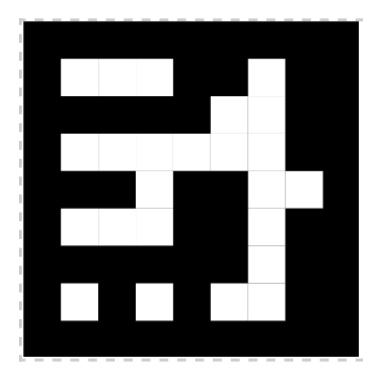
\includegraphics[width=0.2\textwidth]{thesis/marker.eps}
    \caption{Example of generated marker from  \texttt{DICT\_7X7\_50}, ID = 1}
    \label{fig-marker}
\end{figure}
\FloatBarrier
Before their detection, ArUco markers need to be generated then printed in order to be placed in the environment. The OpenCV library has a built-in ArUco marker generator through its cv2.aruco.drawMarker function. The main parameters of this function is the marker dictionary and the ID of the marker which has to be a valid ID in the ArUco dictionary. By specifying the marker dictionary and the marker ID, the drawMarker function then returns the output image with the required ArUco marker drawn on it. 

There are 21 different ArUco dictionaries built into OpenCV. The majority of these dictionaries follow a specific naming convention, \texttt{cv2.aruco.DICT\_NxN\_M}, with an NxN size followed by an integer value, M. For example \texttt{DICT\_6X6\_250} means this dictionary is composed of 250 markers and a marker size of 6x6 bits. There are some settings to consider in order to choose the ideal dictionary, and these differ from system to system. It is generally more ideal to pick a dictionary with a larger NxN grid size, balanced with a low number of unique ArUco IDs such that the inter-marker distance can be used to correct misread markers\cite{opencv-aruco}.
Therefore, for my system, I have chosen the \texttt{DICT\_7X7\_50} (\ref{fig-marker}), because my system requires 15 unique IDs for 15 different actions, and this dictionary has the smallest number of unique IDs (50 IDs). The marker size of 7x7 bits also provides more accurate detection results than other marker sizes due to the larger grid size and inter-marker distance. 
I have generated a total of 15 markers for my system with ID’s in the range of [1,15], with one increment. 

\subsubsection{Detectmarker()}

The OpenCV library is used to detect the markers in the frames rendered by the imutils video library. I have made use of OpenCV’s cv2.aruco module specifically made to detect aruco markers. The marker detection process is comprised of two main steps:
\begin{enumerate}
    \item Detection of marker candidates. In this step, the frame read by the VideoStream.read() function  is analyzed in order to find square shapes that are candidates to be markers. It starts with an adaptive thresholding to segment the markers, then outlines are extracted from the thresholded image and those that do not approximate to a square shape are discarded. Some extra filtering is also applied to removing contours that are too small, too big, or too close to each other.
    \item After the candidate detection, it is necessary to determine if they are actually markers by analyzing their inner codification. This step starts by extracting the marker bits of each marker. The image is divided into different cells according to the marker size and the border size. Then the number of black or white pixels in each cell is counted to determine if it is a white or a black bit. Finally, the bits are analyzed to determine if the marker belongs to the specific dictionary. Error correction techniques are employed when necessary.
\end{enumerate}
I have designed my system to specifically detect markers from the dictionary \texttt{DICT\_7X7\_50} as specified in the previous paragraph. Since my system makes use of a live stream video from the webcam, I have included code to draw the outlines, the center and the ID of the detected tag on the screen to show real time detection. 
Finally, the IDs of the detected markers are stored in a list and used to translate to a flashing light sequence of instructions or parsed to the block recognition code, that plays an audio file depending on the block recognized.

\section{playsound}

To implement the block recognition feature, I have used the playsound Python module. This enables my system to play mp3 audio files describing the action on the block detected by the OpenCV detection algorithm. My code performs this by detecting the marker ID, each marker ID has been assigned to an action. Table \ref{tab-sound} shows examples of markers and their corresponding audio output.
\FloatBarrier
\begin{table}[h]
\centering
\begin{tabular}{|c|c|c|}
\hline
Marker ID      & Action Associated      & Audio Output      \\
\hline
$1     $ & Start program  & $\texttt{'Start Block'}   $ \\
$3     $ & Turn Left      & $\texttt{'Make a Left Turn'}   $ \\
$5     $ &U-turn Left& $ \texttt{'Make a U-turn to the left'} $\\
$7     $ & Move Forward & $\texttt{'Move Forward Block'}   $ \\
$9     $ & Variable Block: 5 steps   & $\texttt{'Move for 5 steps'} $ \\
\hline
\end{tabular}
\caption{Examples of markers and their corresponding actions.}
\label{tab-sound}
\end{table}
\FloatBarrier
\section{Tkinter}

To build my GUI, I have utilised the GUI Python Framework Tkinter and its functions to allow the user to interact with my system.

\subsection{Frame}
My GUI design involves a frame widget, it works on grouping and organizing other widgets by arranging their position. This widget is essential in my system since it allows me to choose the background color and the size of the displayed windows. For example, the parent window, which is the window displayed when the system starts, includes an organised layout of a label widget and different button widgets. The system displays a new frame depending on the buttons clicked. Hence, I have employed the frame widget as a foundation class to implement widgets and different windows.

\subsection{Button}
I have implemented the tkinter button widget in my system. There are two buttons that appear on the main window when the application starts. The buttons are linked to different functions in my code and perform the required actions depending on the button clicked.

\subsection{Label}
The label widget was used to display information such as descriptions or instructions at the top of the screen once the GUI has been loaded. I have also employed this widget to display any error messages that the system detects.

\section{Programming the Ozobot}
To interpret the detected markers and their associated instructions and convert them into flashing light sequence for the Ozobot, I have implemented an open-source Python-like language compiler for Ozobot called Ozopy, invented by Kaarel Maidre\cite{ozopy}. This Python-like language is a subset of Python with some added builtin methods to control the Ozobot Bit.

\subsection{Context}

The Ozobot can be programmed in two ways, either by using color codes and colored markers to indicate actions, or by using the visual programming interface OzoBlockly. With OzoBlockly, the user can create programs for the Ozobot by dragging puzzle shaped blocks onto the programming platform. The on-screen blocks clip together to form a program. The OzoBlockly editor has five skills levels from pre-reader to master.
For my system’s purposes, I will be focusing on level 1 and level 2, which are pre-reader and beginner levels. This is due to there being very few accessible programming interfaces for younger demographics. The level 1 blocks feature simple shapes depicting movements such as arrows, while level 2 blocks feature the same blocks with written statements instead of icons and with the addition of loops. 

To convert the created program into instructions understood by the Ozobot, OzoBlocky displays the encoded values as a light sequence composed of 8 color constants: black, white, red, green, yellow, blue, magenta and cyan. This is scanned at the base of the Ozobot where the RGB colour sensors reside. 

The engineering of the colour codes for OzoBlockly is not publicly available. However, Kaarel Maidre and Ashley Feniello have successfully reverse engineered the colour codes and created Ozopy and FlashForth\cite{ashley}, a programming IDE for the Ozobot. The following section explains the working of Ozopy.  

\subsection{Encoding Values}
Ozopy functions similarly to OzoBlockly. The language compiler interprets a set of instructions written on an .ozopy file and outputs a window with flashing lights  of colour codes. These colour codes translate to bytecode instructions that the Ozobot executes. Ashley Fenielo, who made FlashForth, has successfully decoded the colour sequences and established their corresponding bytecodes\cite{ashley}. Her work represents the groundwork behind Ozopy.
\FloatBarrier
\begin{table}[h]
\centering
\begin{tabular}{|c|c|c|c|}
\hline
\textbf{Denary Value}  &\textbf{Color}  & \textbf{3-bit encoding} &  \textbf{Letter}  \\ \hline
0     &Black &000 &K   \\ \hline
1    &Red   &001 &R            \\ \hline
2   &Green &010 &G               \\ \hline
3    &Yellow  & 011 &Y              \\ \hline
4   &Blue &100 &B                \\ \hline
5   &Magenta &101&M             \\ \hline
6   &Cyan & 110 & C                \\ \hline
7   &White & 111 &W               \\ \hline

\hline
\end{tabular}
\caption{Ozobot color codes and their values\cite{ashley}}
\label{tab-colors}
\end{table}
\FloatBarrier
The color codes are encoded in a base-7 encoding and line up on byte-sized boundaries encoded as sets of three colours. Each of the eight colors has a 3-bit value. Table \ref{tab-colors} shows the denary value of the colors and their 3-bit encoding. A set of three consecutives colors encode a bytecode used to program the Ozobot, except for the color White which is not being used as a value but rather signifies repeating the last color. For example, KWK is simply 000. Each of the three color codes is then translated to a decimal number. The resulting number is converted to hexadecimal to produce a bytecode that can be used to lookup instructions that are featured on the Ozobot. 

\subsection{Instructions}
After the color codes are translated to bytecodes, the resulting bytecode value is used to lookup instructions. As the Ozobot functions as a stack machine, operands are sent before operations.
Values of less than 128 are considered literals pushed to the stack, while values of 128 or higher are instructions. The table created by Feniello shows the bytecodes and their matched instructions. \ref{tab-bytecode}

\subsection{Ozopy language}
The Ozopy language is a python-like language built by Kaarel Maidre. It builds on the work of Ashley Feniello and acts as a compiler that decodes instructions into bytecodes and then translates them into a flashing light sequence. It features several instructions similar to Python synatx such as if, else and while. It also includes Ozobot specific functions such as move, rotate. The functions provided by the language are shown in table \ref{tab-ozopy}

\begin{table}
\centering
\begin{tabular}{|c|c|l|}
\hline
\textbf{Bytecode}  &\textbf{Instruction}  & \textbf{Explanation}  \\ \hline
0x80 &if & \\ \hline 
0x85 &+  &\multirow{5}{*}{Arithmetic operations}\\ 
0x86 &- & \\ 
0x87 &*  &    \\ 
0x88 &/   &   \\
0x89 &mod  &  \\ \hline 
0x8a &not   &Boolean \\ \hline 
0x8b &neg &Reverse sign\\ \hline 
0x8c &rand &Random integer from X to Y \\ \hline 
0x90 &call &\\ \hline 
0x91 &; &Return\\ \hline 
0x92 &get/sensor &Get variable/sensor\\ \hline 
0x93 &set &Set the value of a variable\\ \hline 
0x94 &dump &\\ \hline 
0x96 &drop &Pop only one value\\ \hline 
0x98 &turn &Rotate Ozobot by X degrees at Y mm/s. e.g. 180 50 turn\\ \hline 
0x9b &wait &Wait for X centiseconds. e.g. 64 9B waits for one second (64 hex = 100decimal)\\ \hline 
0x9c &\textgreater = &\multirow{2}{*}{Comparisons}\\ 
0x9d &\textgreater &\\ \hline 
0x9e &move &Move Ozobot by X mm at Ymm/s. Example: 100 50 turn\\ \hline  
0x9f &wheels &Set wheel speeds individually\\ \hline 
0xa2 &and &\\ \hline 
0xa3 &or &\\ \hline 
0xa4 &= &\\ \hline 
0xa5 &pick &Get value from stack at specified depth, values are not consumed.
\\ \hline 
0xa6 &put &\\ \hline 
0xa7 &pop &Pops values off the stack\\ \hline 
0xa8 &abs &Absolute value\\ \hline 
0xae &end  &end of execution\\ \hline 
0xb8 &led  &Sets color of LED\\ \hline 
0xba &jump  &Branching \\ \hline 
0xc7 &kill &Causes starter pack Ozobots to die \\ \hline 

\hline
\end{tabular}
\caption{Ozobot color codes and their values\cite{ashley}.}
\label{tab-bytecode}
\end{table}

\begin{table}
\centering
\begin{tabular}{|c|l|}
\hline
\textbf{Instruction}    & \textbf{Explanation}  \\ \hline

=                       & \multirow{6}{*}{Arithmetic operations}\\
+                       &                           \\ 
-                       &                           \\ 
*                       &                           \\ 
/                       &                           \\ 
\%                      &                          \\ \hline
random(low, high)       & Generate a random value wihtin the given range                         \\ \hline
abs(value)              & absolute value of the given parameter                     \\ \hline
move(distance, speed)   &Move forward Xmm at Ymm/s \\ \hline
rotate(angle, speed)    &Rotate X degrees at Ymm/s \\ \hline
wheels(left, right)     &Set each wheel speed individually. Wheels(0, 0) stops the robot                                         \\ \hline
follow\_line\_to\_intersect\_or\_end()  &Follows a line drawn on the surface \\ \hline
move\_straight\_until\_line(speed) & Moves forward at a given speed until it reaches a line  \\ \hline
there\_is\_way(direction) &\vtop{\hbox{\strut Checks for a line in a given direction. Direction can be STRAIGHT, LEFT, }\hbox{\strut RIGHT or BACK.}} \\ \hline
pick\_direction(direction) &Chooses a particular direction when the Ozobot reaches an intersection \\ \hline
set\_line\_ speed(speed)   &Sets the line following speed \\ \hline
get\_line\_speed()    &Gets the current set line following speed \\ \hline
get\_intersect\_or\_ line\_end\_color()   &Read the colour of the line the robot is following \\ \hline
get\_surface\_color() &\vtop{\hbox{\strut Get colour of surface below Ozobot,Color can be BLACK, WHITE, GREEN,}\hbox{\strut RED, BLUE, YELLOW, CYAN and MAGENTA}} \\ \hline
color(red, green, blue)     &Set the value of the LED on top of the robot. Color(0, 0, 0) turns the LED off.\\ \hline

wait(seconds, centiseconds) &Waits for specified time\\ \hline
terminate(mode)     &\vtop{\hbox{\strut Ends program. Mode can be one of three specified constants, OFF, FOLLOW,}\hbox{\strut or IDLE.}}\\ \hline
if else &\\ \hline
while               &Only while is supported for loops\\ \hline
def                 &Create functions. Cannot have return values or parameters\\ \hline
          


                     

\hline
\end{tabular}
\caption{Ozopy Language\cite{ozopy}}
\label{tab-ozopy}
\end{table}



% -----------------------------------------------------------------------------
\chapter{System Design}
\label{chap:design}
In this section, I will describe the iterative design process I have used to create my final system. The system design was completed in the following steps:

\begin{enumerate}
    \item Design an initial prototype based off the studied works.
    \item Present the prototype to experts in the field and co-design with them to improve the prototype.
    \item Test the revised prototype with end users and make the required changes.
    \item Implement a final improved design.
\end{enumerate}


\section{Initial Design Concept}
\begin{figure}
    \centering
    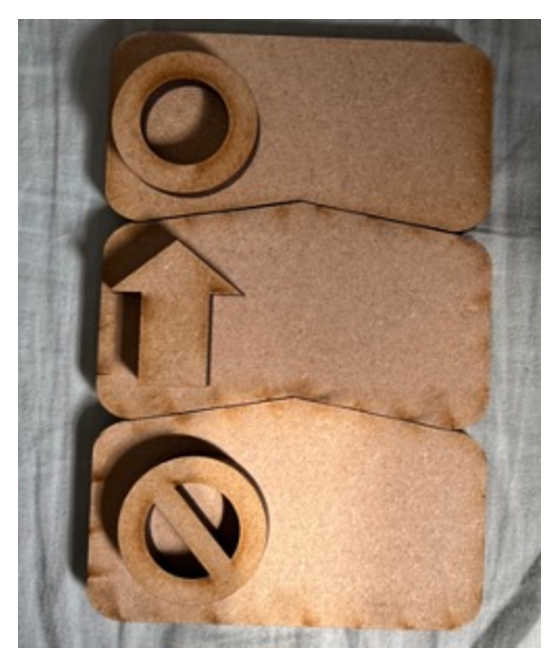
\includegraphics[width=0.3\textwidth]{thesis/initial-block.eps}
    \caption{Initial Prototype, with Go symbols, go forward, and end symbol}
    \label{fig-initial}
\end{figure}
I created my system with the aim to be an accessible platform to program the Ozobot, that children with mixed visual abilities could use with their teachers in classrooms or with friends, to learn basic concepts of programming. This aim meant that I followed an iterative design process and set some initial design decisions before I engaged in the co-design process with experts. My initial design was based off the advantages I identified in publicly available TUI and other works that I discussed in previous sections.

My first decision was to utilize passive blocks to reduce the cost and simplify the manufacturing process, while enabling more flexibility in shapes and sizes, inspired by StoryBlocks\cite{storyblocks}.  Active programming blocks such as Torino pods may be advantageous for interactivity, but they are difficult to manufacture, bulkier, more expensive and less robust than passive blocks\cite{torino}.  Each block represents one component, including actions, loops, and variables. Each block features a 3D icon on top of it for the students to recognise the action that each block depicts. The tactile icons ensure that my system is accessible to mixed visual abilities.

My second design decision was to use a camera and a series of fiducial markers for block recognition, due to the fact that camera-based systems for marker recognition are inexpensive, robust and easy to implement on mobile, online and desktop applications.

To manufacture my initial prototype, I have experimented with different materials. I had considered utilizing acrylic, as it comes in different colors and that would be helpful for children with low vision to distinguish between different blocks. However, acrylic material proved to be heavier and less robust than other alternatives. Additionally, I experimented with laser cutting and making blocks out of MDF and plywood. Plywood was the better option, it is less heavy than MDF and less susceptible to damage. 

Thus, I created an initial prototype \ref{fig-initial} with blocks made from 6mm thick plywood and are 10cm wide and 5cm high. I chose the material and size with the aim of having light but robust blocks, with a size that would be easy for children to pick up and move around.


\section{System Design with Experts}
To inform the design of my system, I interviewed a Special Educational Needs teacher (SEN) and a qualified teacher of the visually impaired (QTVI), both had extensive experience in teaching and mentoring visually impaired children. The participants were involved in the design process for their knowledge of the difficulties that VI children face with programming, especially in light of their outreach and mentoring experiences. Both interviews were semi-structured and conducted separately.

The participants gave feedback on my initial design prototype and explored other mechanisms for interaction, in order to identify the ideal design features for the tangible blocks. The interviewees also defined design requirements for the workspace of the system and suitable activities for trial sessions with children. 
The interviews were audio recorded and fully transcribed to extract design recommendations for the system using thematic analysis [10]. Thematic analysis was carried out using an inductive approach and the construction of themes was guided by three research questions: 
\begin{itemize}
    \item How would the characteristics of the blocks modulate how the children interacted with them and with each other?
    \item How would the system's workspace support children in building programs as they engaged with the activities? 
    \item What activities would my system utilise to help children gain an understanding of computational concepts and practices?
\end{itemize}
Here, I will summarize the main themes and insights I have gained from these sessions.

\subsection{Tactile Features}
The participants first examined my initial prototype and identified features to improve on.
\subsubsection{Block Shape and Size}
Firstly, the participants both agreed that the blocks should be small and confirmed that the prototype was a good size. The fact that the blocks are small and light makes it easy for  children with mixed visual abilities to use them and may help them develop their fine motor skills. The QTVI also mentioned that the  matching concave and convex shapes in my prototype to make the blocks fit together might be confusing for children who are visually impaired, and that it would be best to utilise a rectangular shape, as they are more accustomed to basic shapes and could recognise it immediately by tact. Additionally, both participants were attracted to my suggested idea of incorporating magnets in the blocks to clip them together. They explained how VI children tend to move objects around a lot to explore haptically, hence a mechanism to keep blocks together would be very useful.

\subsubsection{Symbols}
The participants concurred that the best way to convey the meaning of the blocks to the children is by using icons. They should be easily-recognizable and need to be embossed or in 3D and with minimalist design. The symbols should also be put on top of the blocks as this would make the blocks more intuitive and easier for VI children to touch and recognise symbols.
I presented different icons to associate with different actions, such as arrows for directions and circles for a start block. The QTVI agreed that simple icons such as shapes are easily recognisable for VI students, and that too much information is distracting. The use of arrows and circles is ideal, as long as the arrows are acute enough to show that direction they are pointing and the lines on the icon are 6mm apart to allow VI students to distinguish them tactually. Additionally, the SEN mentioned that visually impaired children can recognise patterns tactually, so it would be useful to use similar shapes if they mean similar types of actions. For example, using different types of arrows for directions, or using a circle for the start block to start the program and a circle with a line going through it for the end block to end the program. It would not only make the system easier to use but would also teach the children the computational concept of pattern recognition.

\subsubsection{Orientation of the blocks}
Correctly orientating the block is very important for my system's functionality. Thus, it was a theme that was also explored during interviews. The SEN teacher suggested using bumpons, self adhesive dots that are great for marking objects. They confirmed that if a bumpon is placed on the top left hand corner of the block, then visually impaired children would identify the correct orientation of the block. It is a commonly used orientation technique in schools.
\subsubsection{Function Blocks with variables}
Another important design decision was to identify a suitable way to enable children to combine instruction blocks for the robot, such as Go forward/backwards and loops, with variable blocks indicating different numbers of steps or loop iterations. I discussed various ways with my interviewees to combine these blocks using magnets, matching concave and convex shapes or shapes that could slot into each others. They preferred variable blocks slotting inside the instruction block, for several reasons. Firstly, this method suggests a better conceptual representation of the relationship where the variable modifies the execution of the Move forward/backward or repeat functions. Secondly, it provides immediate tactile distinction between the smaller variable blocks and larger hollow function blocks. Finally, having blocks slot into each other would prevent them from accidentally separating, making it easier to manipulate the code sequence.
\subsubsection{Loop Blocks}
Next, I had to decide how to present functionality, such as loops, that could be expanded to contain other blocks.  Block-based languages such as Scratch usually represent loops by a larger block that stretches to contain instructions nested inside \cite{scratch}.
The QTVI suggested that loops have a start and an end loop block. Similarly to the circle icons for start and end program blocks, it was suggested for the end-loop blocks to be similar to the start-loop blocks to facilitate the conceptual link between the two blocks without causing confusion.
\subsubsection{Variable Blocks}
To represent the value of variables, I explored different tactile features including dots, lines or using Braille.
The participants preferred dots over other alternatives to invite counting as many VI young children are not proficient in braille. Additionally, it would be hard for the VI user to count lines if they are not sufficiently spaced. For my design to be as small as possible, dots are the best approach, although the participants recommended they be placed 6mm apart to allow for tactile recognition and to avoid configurations that resembled braille cells, which could be confusing for some children. The QTVI expressed that embossed features were also generally found easier to read compared to engraved ones, especially when counting the number of dots in a variable. The SEN teacher also suggested sticking bumpons on the block for counting. Because bumpons come in a variety of shapes, a shape other than the one used for block orientation can be used for variable counting.
\subsubsection{Block Color}
As my system is aimed at children with mixed visual abilities, the participant suggested that I incorporate design features to support both tactile and visual learners. Specifically, it was decided that blocks should have a good color contrast with the symbols, by having the icons painted black and the rest of the block in its neutral color. Tactile features painted in high contrast on the blocks make it easier for children with partial or complete vision to recognise them visually.

\subsection{Designing the Workspace}
Once the features of the blocks had been defined, it was important to discuss characteristics of the workspace. It was essential to have a defined workspace in my system to indicate to students where they should construct sequences of code. This is particularly useful for visually impaired users who would tactually identify an outlined workspace to create a mental map of the environment, as it aids them in placing the blocks and performing debugging operations. As the system utilises a webcam to scan the blocks, the webcam would also be a part of the workspace and would be placed above it to have a full view. Both participants suggested utilising rectangular trays, which are often used in tactile exploration sessions with VI children in schools. I suggested outlining the workspace with Lego to provide the children with tactile cues to identify the programming space, as well as have a expandable workspace frame. The participants agreed that this would be a good strategy, and that making the workspace size adaptable would allow for more blocks.
Finally, to prevent the blocks from moving around on the workspace, the participants suggested to use Dycem, which is a non slip grip material, that prevents objects placed on top of it from shifting. This would ensure that the code sequence on the workspace is intact and ready to be scanned by the webcam.

\subsection{Collaborative Learning}
My system aims to be a TUI inclusive of children with different visual abilities, rather than being specifically designed for fully blind children. To promote collaborative learning between mixed visual abilities, I aimed to make my system accessible to all in a number of different ways. My expert participants recommended using high contrast to highlight the presence of dots and icons, to make the system more accessible to partially sighted children. They also agreed that including Braille could create confusion for sighted children, or the many VI children who were not braille literate and could isolate them from others rather than promote inclusion. Thus, no braille description will be added to my blocks.

The symbols I initially chose for my system are symbols commonly found on devices or encountered in every day life, my participants confirmed that it would be easy for students to recognize the symbols, once they were explained their meaning. Furthermore, the idea of using symbols commonly associated with the indicated actions, such as arrows for directions, was received positively as it would build on the affordances of the teachers, and sighted or partially sighted children, facilitating inclusion and shared play.

\subsection{Activities and Goals}
The final part of the interview was spent discussing activities for the testing session and future improvements for my system. For the initial design iteration, the aim of my system is to introduce three basic computational concepts: sequences, loops and data, and support the computational practices of being iterative and incremental; and testing and debugging. I left out more complex computational concepts such as conditionals and operators from my design as they could increase the complexity of the system. 

Once the participants were familiar with the working of my system, they suggested activities to test the TUI with mixed visual abilities. The SEN teacher suggested turning symbol recognition into a game before introducing the programming aspect of the system. They explained that by getting the students to physically move in space, and pretend to be the Ozobot going in different directions they can turn the abstract idea of coding the robot to something concrete, and in turn understand the meaning of the symbols on the blocks better. When it comes to programming tasks, the participants explained that VI children learn about routes in schools and have a good understanding of spatial navigation. Thus activities that involves paths or routes for the robot to follow are ideal. Sound output is also important for the children to monitor their success. Hence, I proposed including external elements, such as towers of wooden blocks that are knocked down as the robot completed different segments of the path, allowing visually impaired children to monitor the robot's location.

\section{Final Design Requirements}
In this section, I will summarise the final design requirements for my system. The final design incorporates the insights provided by the co-design process with the QTVI and the SEN teacher and the findings gathered from relevant literature. These  requirements provide the basis for my final system implementation, that will be detailed in chapter 6.

The final design requirements can be summarised in Table \ref{tab-blocks} for the blocks and Table \ref{tab-workspace} for the workspace.

\FloatBarrier
\begin{table}[h]
\centering
\begin{tabular}{|c|l|}
\hline
\bf Design Components       &\bf Design Requirements        \\ \hline
\text{Geometry}       & \text{Rectangular shaped blocks, small size}  \\  \hline
\text{Material}    & \text{Light and Robust material, e.g. plywood}  \\ \hline
\text{Icons}  & \text{Simple 3D icons  embossed on top of blocks with 6mm gaps between outlines}    \\ \hline
\text{Instruction blocks} & \text{Blocks with embossed icons and fiducial marker on top} \\ \hline
\text{Function blocks} & \text{Loops, move forward/backwards blocks. Include slotting for variable input} \\ \hline
\text{Variable blocks} & \text{Smaller sized blocks that are slotted into function blocks, with embossed dots for counting.} \\ \hline
Combining Blocks &Clip blocks together using magnets to prevent them from seperating \\ \hline

\text{Color}       & \text{High color contrast between symbols and blocks.}   \\ \hline


\hline
\end{tabular}
\caption{Final Design Requirements for Blocks.}
\label{tab-blocks}
\end{table}

\begin{table}[h]
\centering
\begin{tabular}{|c|l|}
\hline
\textbf{Design Components}       & \textbf{Design Requirements}    \\ \hline
Bounds     & Workspace bounded with a rectangular tray or Lego.  \\ \hline
Surface    &Include a non-slip material on the surface to prevent blocks from slipping. \\ \hline
Webcam   & Webcam propped with a tripod high enough to view the workspace. \\ \hline
Size    &Adaptable size to fit a maximum of blocks. \\ \hline
Map  & Map with a route for Ozobot to follow, includes audio feedback.    \\ \hline

\hline
\end{tabular}
\caption{Final Design Requirements for Workspace.}
\label{tab-workspace}
\end{table}
\FloatBarrier



\section{Design Workshop}
As the next step in my iterative design process, I set out to create more prototypes of my blocks in order to test different designs with users. 
Due to multiple viable design decisions, the design workshop aimed to answer questions that were left unanswered after the expert interview. The explored themes are described below. 
Participants were shown and tested various possible designs in order to gather feedback and determine final design requirements for a final implementation. 
The research was audio recorded, and transcripts were created to document the main design outcomes.
\begin{enumerate}
    \item What action do you associate with the presented symbols?
    \item How would you combine function blocks with variable blocks?
    \item How would you put blocks together?
   
    
\end{enumerate}
\subsection{Participants}

Seven participants partook in my study. All participants fit the participation criteria, which required the person to be over 18, have limited experience coding robots and are a student. No participants had any disability or impairment. I conducted the design workshop in person in a group setting to create a dynamic conversation and allow other members to express their opinions on the design and counter or approve each other's opinions. The study also aimed to determine the system's best features, so a group discussion would result in a final design decision based on the majority's opinion.  
All participants were recruited by online communications. Each participant was given a Participant Information Sheet before the study that detailed the interview process and what was required if they chose to take part. If the participant consented to proceed with the study, the consent forms were handed over and signed in-person.

\subsubsection{Recruitment Note}
Recruitment of visually impaired students was attempted on relevant social media groups. I successfully recruited one VI individual, however due to COVID, the participant was unable to complete the study in the required time frame. Designing my system without a key demographic (VI) resulted in the design results not being as relevant as they possibly could. Thus, I will utilise the input of the SNE and QTVI gathered in the previous section as a guideline on the design requirements for VI individuals, in an attempt to mitigate this limitation.

\subsection{Results}
In this section, I will discuss the different outcomes of each question.

\subsubsection{Question: What action do you associate with the presented symbols?}
The participants were presented with different symbols that I have laser cut into wood. These icons were designed to convey the meaning of each of the blocks. This question aims to see if the participants can guess the associated action. If they cannot, the answer was given to them and feedback about potential improvements on the design were gathered. This step is important to determine if sighted users can use the system independently.
%\FloatBarrier
%\begin{figure}[h]
 %   \centering
  %  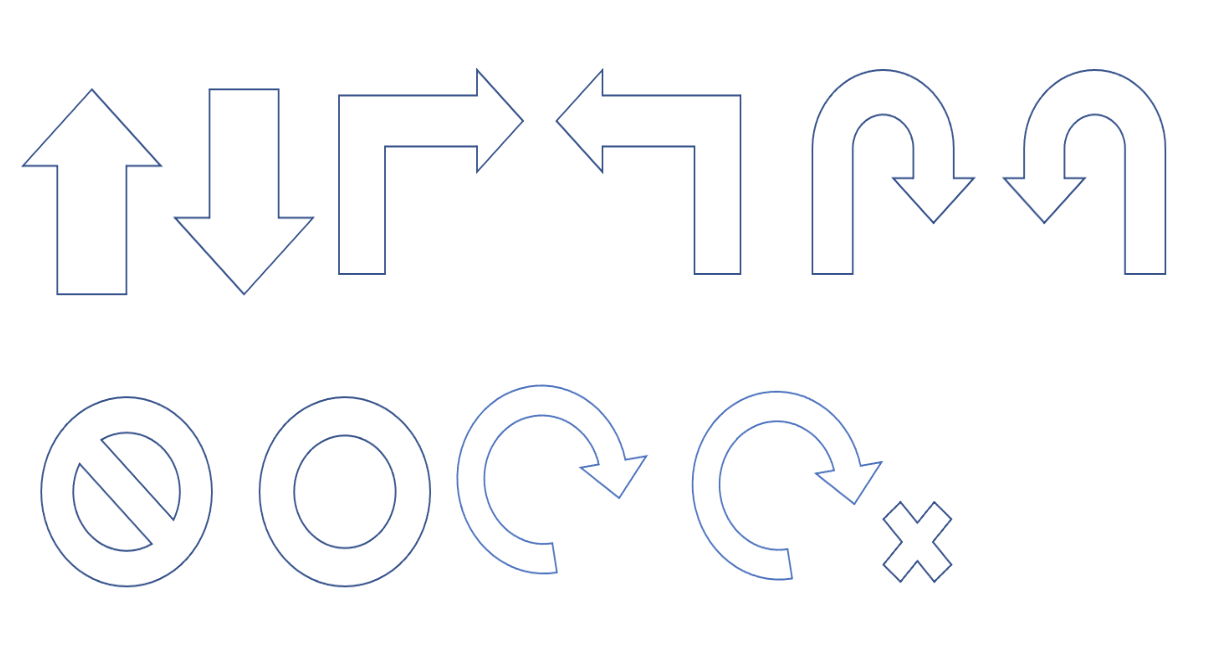
\includegraphics[width=0.5\textwidth]{thesis/design.eps}
   % \caption{Initial Designs of Symbols on CorelDraw}
    %\label{fig-design-initial}
%\end{figure}
%\FloatBarrier
\subsubsection{Go Forward and Go backwards}
All participants associated the symbols in figure 1 and 2 with the go forward and go backwards actions, respectively. The general comments were that the orientation of the icon relative to the participant helped the user understand the action. 

\subsubsection{Turn 90 degrees Left and Turn 90 degrees Right}
\FloatBarrier
\begin{figure}[h]
    \centering
    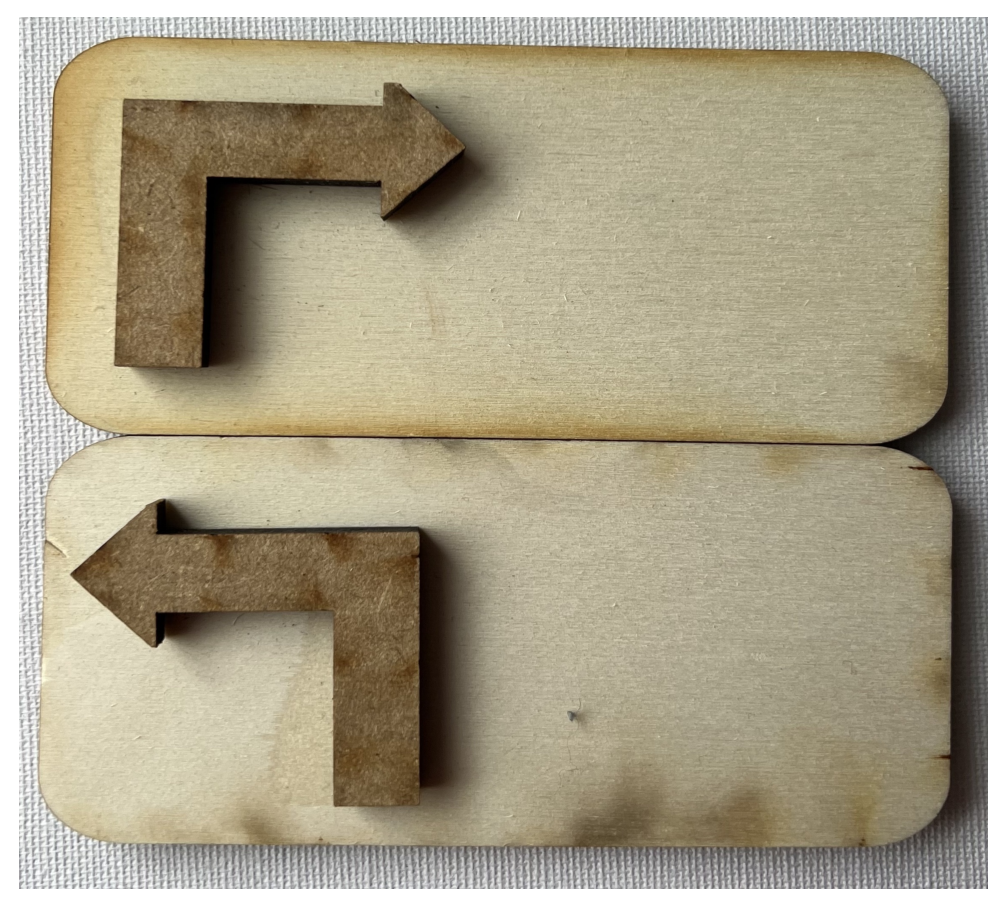
\includegraphics[width=0.3\textwidth]{thesis/turns.eps}
    \caption{'Turn Right' and 'Turn Left' Symbols}
    \label{fig-turn}
\end{figure}
\FloatBarrier
The participants successfully guessed the action depicted by the symbols. They discussed that the 90 degrees angle and the arrow pointing in different directions after a straight line depicts a clear turning action. 

\subsubsection{U-Turn Left and Right}
\FloatBarrier
\begin{figure}[h]
\centering
\begin{minipage}{.5\textwidth}
  \centering
  \includegraphics[width =.5\textwidth]{thesis/uturns.eps}
  \caption{U-turn Symbol}
  \label{fig:initial-turn}
\end{minipage}%
\begin{minipage}{.5\textwidth}
  \centering
  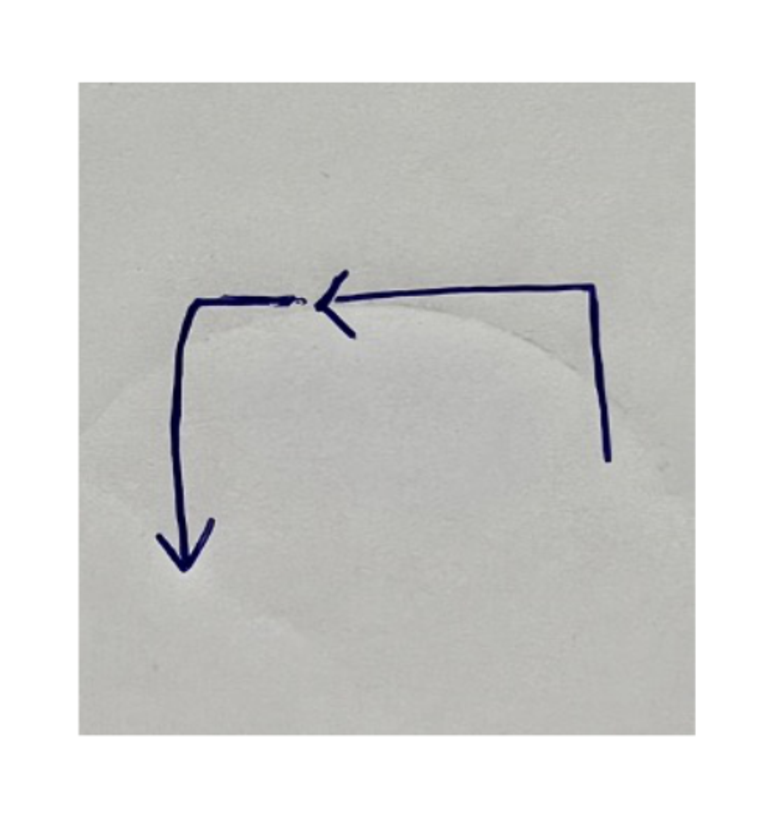
\includegraphics[width=.5\textwidth]{thesis/uturn.eps}
  \caption{Suggested u-turn design}
  \label{fig:suggested-turn}
\end{minipage}
\end{figure}
\FloatBarrier
The seven participants guessed the action correctly, commenting that the curved arrow was similar to that of the u-turn traffic sign and thus easy to recognise. One participant discussed the possibility of combining two left turns or two right turns arrows to depict a u-turn, as shown in his drawing on figure \ref{fig:suggested-turn}. However, the majority of participants protested that it might be confusing for visually impaired children to have two arrows that close to each other and that it resembled the Turn 90 degrees symbols. Another participant commented that it would also take up a lot of space on the blocks.

\subsubsection{Start Blocks}
\FloatBarrier
\begin{figure}[h]
    \centering
    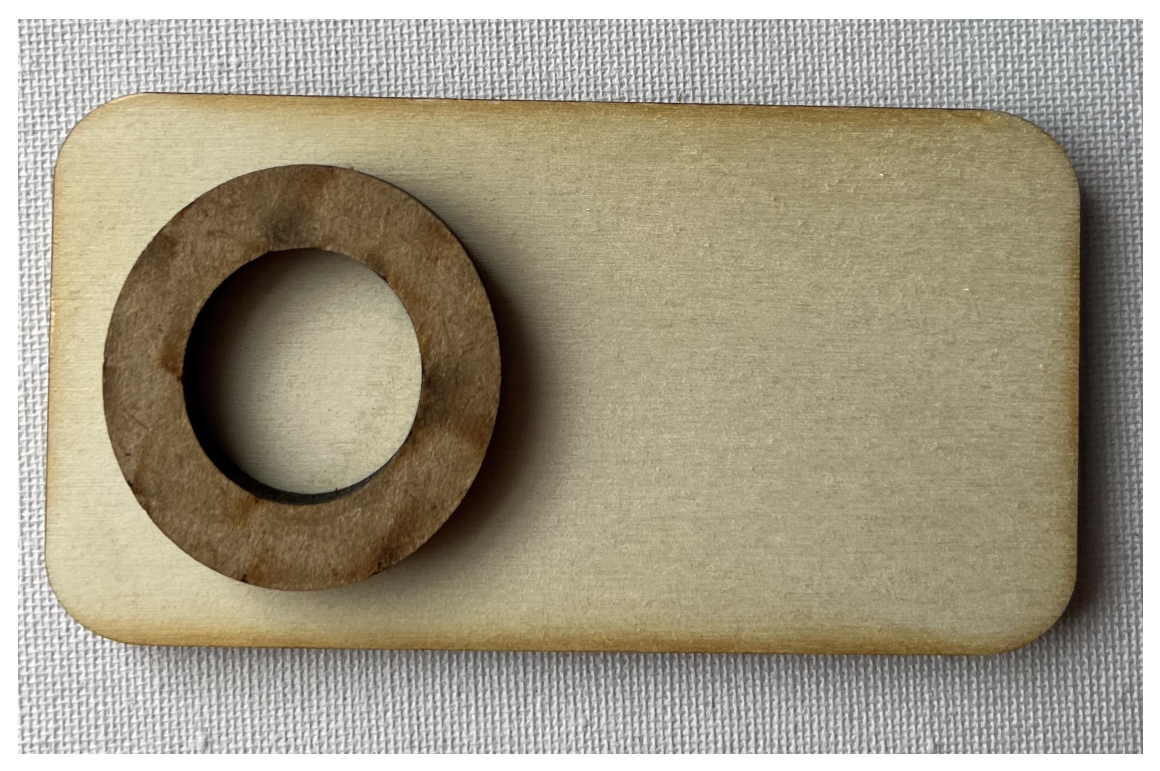
\includegraphics[width=0.3\textwidth]{thesis/start.eps}
    \caption{'Start Program' Symbol}
    \label{fig-start-initial}
\end{figure}
\FloatBarrier
In this case, participants took longer to answer than with other blocks. One participant deduced that the circle resembles the shape of the Go sign used in traffic and concluded that it could be a go or start sign. Four of other participants agreed but two participants remained unsure.  I confirmed that the symbol does in fact relate to the start action. One participant felt that other alternatives should be explored, such as using a triangle, like the play button to convey the 'start' meaning. However, it was decided that this required too much explanation and the use of a triangle may be confused with the arrows.

\subsubsection{End Block}

\FloatBarrier
\begin{figure}[h]
    \centering
    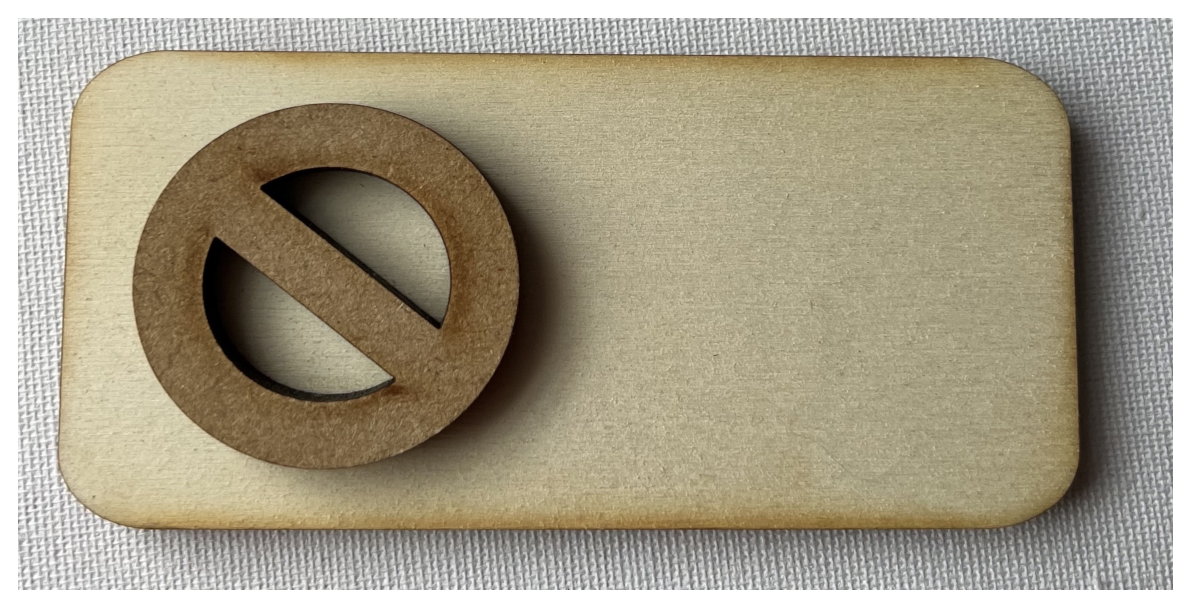
\includegraphics[width=0.3\textwidth]{thesis/end.eps}
    \caption{'End Program' Symbol}
    \label{fig-end-initial}
\end{figure}
\FloatBarrier
After examining the start symbol, it was much easier for participants to guess the meaning behind the stop symbol. All participants understood the meaning of the symbol correctly. One participant mentioned using a cross symbol instead due to the fact that the children may be unable to understand the icon if they are unaware of road signs. However, four participants mentioned that a cross may be confused with other meanings, such as cancel, or may be mistaken for arrows by visually impaired students. One participant expressed that the teacher could explain the concept of road signs to the child before beginning the task, allowing them to understand this symbol and previous ones. All participants agreed to use the presented symbol, a circle with a line through the centre, as it was the most ”universally understood” symbol. 

All participants mentioned that they related the start symbol to the stop symbol. With the line going through the circle, it was easy to match the pattern to the start symbol and deduce the stop action. From the responses to this question, I concluded that the symbols relate like I planned to and it was easier to recognise them after recognising the pattern i.e. the circle. 

\subsubsection{Start-Loop Block}

\FloatBarrier
\begin{figure}[h]
    \centering
    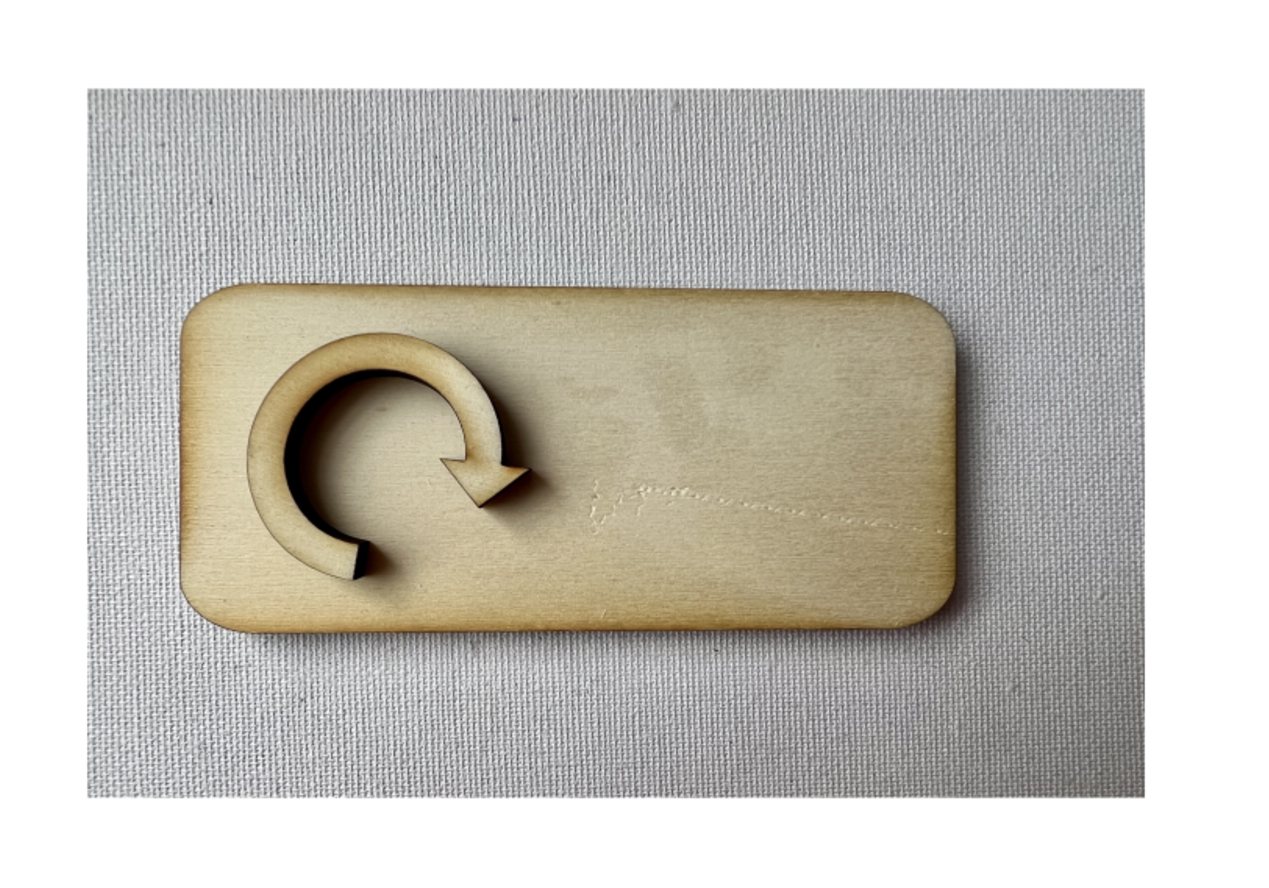
\includegraphics[width=\textwidth]{thesis/loopstart.eps}
    \caption{'Start-Loop' Symbol}
    \label{fig-startloop}
\end{figure}
\FloatBarrier
In this case, all participants struggled to understand the meaning of the symbol in \ref{fig-startloop}, with five participants interpreting it as a 'rotation' action. One participant voiced that they thought it resembled a 'redo' or 'undo' symbol. I explained that the real meaning behind the symbol is a loop or repetition. As this icon was majorly misinterpreted, I gathered feedback about other potential designs. All participants drew suggestions using pen and paper, and then the designs were compared and discussed in a group. The common theme was a circular icon and arrows, one participant drew a spiral with an arrow at the end \ref{fig:sub1}, others drew two arrows pointing at each other. We had a group discussion to determine the best icon. Other participants commented that the spiral design as seen on , could be confusing and hard to recognise tactually. Additionally, laser cutting a spiral would take up too much space on the block. As for the design shown in \ref{fig:sub2} , other participants felt that it could be mistaken for the u-turn symbol like the initial design. Most of the participants agreed that design \ref{fig:sub3} and design \ref{fig:sub4} accurately portray the meaning of 'repeat' the best. The final design decision was to use design \ref{fig:sub4}, as participants felt two semi-circles and arrows would save more space and also goes in theme with the 'loop' meaning.
\FloatBarrier
\begin{figure}[h]
\centering
\begin{subfigure}{.2\textwidth}
  \centering
  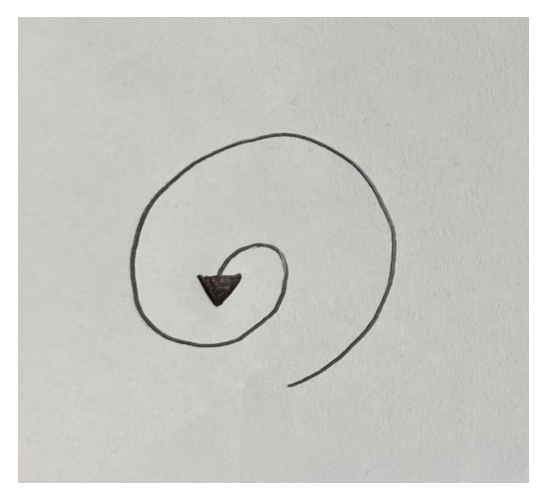
\includegraphics[width=\textwidth,height=3cm]{thesis/spiral.eps}
  \caption{}
  \label{fig:sub1}
\end{subfigure}%
\begin{subfigure}{.2\textwidth}
  \centering
  
\includegraphics[width=\textwidth,height=3cm]{thesis/spotify.eps}
  \caption{} 
  \label{fig:sub2}
\end{subfigure}%
\begin{subfigure}{.2\textwidth}
  \centering
  
\includegraphics[width=\textwidth,height=3cm]{thesis/repeat2.eps}
  \caption{}
  \label{fig:sub3}
\end{subfigure}%
\begin{subfigure}{.2\textwidth}
  \centering
  
\includegraphics[width=\textwidth,height=3cm]{thesis/repeat.eps}
  \caption{}
  \label{fig:sub4}
\end{subfigure}
\caption{Shapes created by participants}
\label{fig:test}
\end{figure}
\FloatBarrier
\subsubsection{End-Loop Block}
\FloatBarrier
\begin{figure}[h]
    \centering
    \includegraphics[width=0.3\textwidth]{endloop.eps}
    \caption{'End Loop' Symbol}
    \label{fig-endloop}
\end{figure}
\FloatBarrier
The end-loop block as quickly recognised by the participants as it features the previous symbol with an 'X' next to it. One participant suggested using the end symbol used in the end block, to stick to one symbol meaning 'stop' or 'end'. The other users agreed that relating the symbols together would be beneficial as students would have to remember less icons and their meanings.

\subsubsection{Variable Block}

\FloatBarrier
\begin{figure}[h]
    \centering
    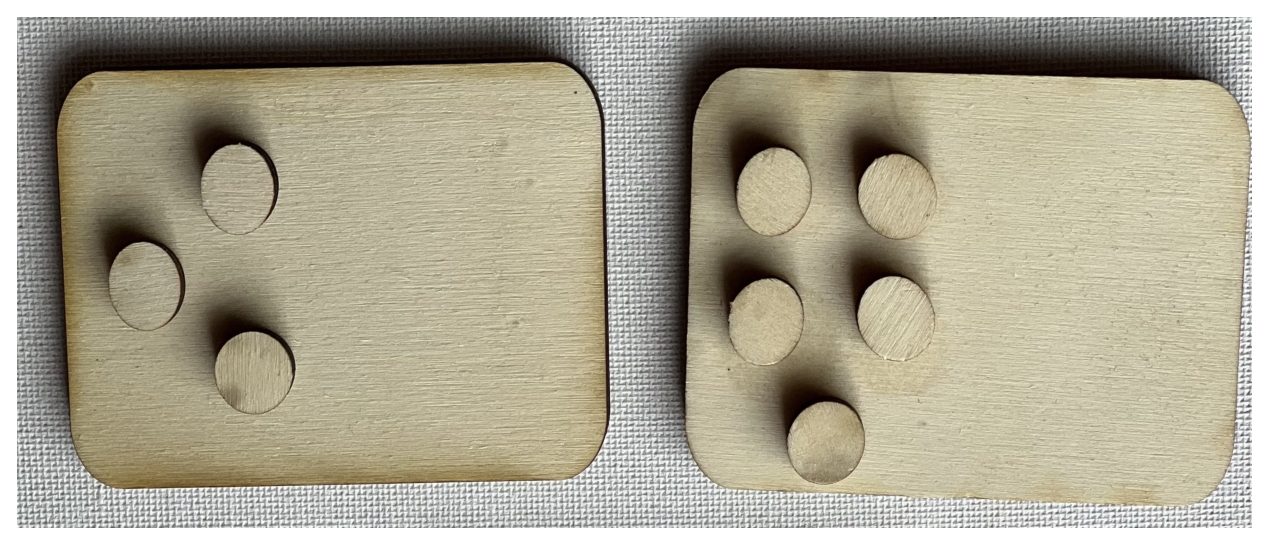
\includegraphics[width=0.4\textwidth]{thesis/variables.eps}
    \caption{Different variable blocks}
    \label{fig-variable}
\end{figure}
\FloatBarrier

The participants understood the meaning behind the variable blocks. Some users compared it to a 'domino', or dice. The general feedback was that the dots were a clear indication of numbers and invite the user to count them.

\subsubsection{Question: How would you combine function blocks with variable blocks?}

\FloatBarrier

\begin{figure}[h]
\centering
\begin{subfigure}{.5\textwidth}
  \centering
  \includegraphics[width=\textwidth]{thesis/hollow.eps}
  \caption{Prototype A: Hollow Function Block}
  \label{fig-hollow}
\end{subfigure}%
\begin{subfigure}{.5\textwidth}
  \centering
  \includegraphics[width=\textwidth]{thesis/engraved.eps}
  \caption{Prototype B: Engraved Function Block} 
  \label{fig-engraved}
\end{subfigure}
\caption{Function Blocks}
\label{fig-function}
\end{figure}
\FloatBarrier

For this part of the study, participants were presented with two different prototypes that satisfy the design requirements for function blocks. The design process with experts specified that the function blocks (i.e. Go Forward/Backwards, loops) should have slots for variable blocks to be fit in, to specify the number of steps or repetitions. The following prototypes were made to satisfy that design decision.


Figure \ref{fig-hollow} represents a function block with a hollow shape to fit the variable blocks. Figure \ref{fig-engraved} represents a function block that has been engraved in the area where variable blocks will be placed. 
The participants experimented with utilising both blocks and picked up variable blocks to fit in them. 
The general consensus was that Prototype (B) was preferred to Prototype (A) for the following reasons. Firstly, participants stated that it was difficult to fit the variable blocks in and even harder to remove them from Block (A) \ref{fig-hollow}, with some participants having to push the variable block from the bottom to pop it out of its position. However, with Block (B) \ref{fig-engraved}, it was engraved deep enough to put the variable block on top without it shifting and it was easy to take the block out, as it was not fully inserted in the function block. Secondly, one participant commented that the hollowness in the first block might be confusing to visually impaired people because there is nothing to tactually explore in that area. On the other hand, Block (B) has a different texture on the engraved surface, which visually impaired students can recognise by touch. In fact, the participant's comment corresponds to the QTVI's assertion that VI people are frequently taught to distinguish between objects by applying different textures to disparate objects. The difference in texture would alert the VI child to the fact that that section of the block is distinct from the rest, allowing them to recognise it as the variable block location.
For those reasons, I have decided to use Prototype (B) \ref{fig-engraved} in my final implementation.

\subsubsection{Question: How would you put blocks together?}
In this part of the study, the participants were asked to experiment with clipping blocks together, using two different sets of blocks. One set of puzzle pieces had magnets on both sides of the blocks and the other was a simple block with no magnets.
The group put 4-5 blocks together for each type.
All the participants were attracted to the first type of blocks due to the magnets that eased the task of attaching blocks. The participants reported that the absence of magnets created gaps in their code sequence and made it difficult to keep blocks together. For this reason, magnets were incorporated in all blocks.


\section{Design Changes}
To summarise, the design workshop built my confidence in certain design decisions while also assisting me in identifying design flaws, such as the loop symbols. The workshop also revealed that some user may struggle to understand the meaning of some symbols when first introduced to the system. Thus, I have added a block recognition feature in my software, that delivers an audio output describing the symbol and the action on the block. This allows children with mixed visual abilities to use the system without prior knowledge about certain signs. The main design changes are:
\begin{itemize}
    \item Change the start-loop and end-loop symbols to the suggest design.
    \item Adopt an engraved block for all function blocks.
    \item Incorporate magnets in the blocks to help clip them together.
\end{itemize}


% -----------------------------------------------------------------------------




% -----------------------------------------------------------------------------
\chapter{System Implementation}
\label{chap:implementation}

Based on the advantages of the existing systems discussed in chapters \ref{chap:context} and my iterative design process with experts and the students in chapter \ref{chap:conclusion}, I designed a tangible Ozobot programming system. In this chapter, I present the implementation of the different components of my system.

\section{Architecture}
My system is composed of a set of tangible programming blocks, an Ozobot robot, a computer application, a webcam with a tripod, and a workspace. Students can manipulate the tangible blocks to construct a program with the desired actions for the robot to execute. The blocks are placed in the workspace underneath the webcam device held by the tripod. The webcam is connected to a computer, where the designed application can recognize the ArUco marker in the blocks and translate them to a flashing light sequence. The Ozobot is held up to the screen to scan the flashing light and then execute the dictated actions. Alternatively, the system can execute the ‘Recognise Block’ feature. This is a separate action that does not program the Ozobot, instead the system uses the OpenCV fiducial marker detection algorithm to detect the blocks and play an audio file describing the action that the block represents. Figure \ref{fig-flowchart} represents the process of the two aforementioned system functions.
\FloatBarrier
\begin{figure}[h]
    \centering
    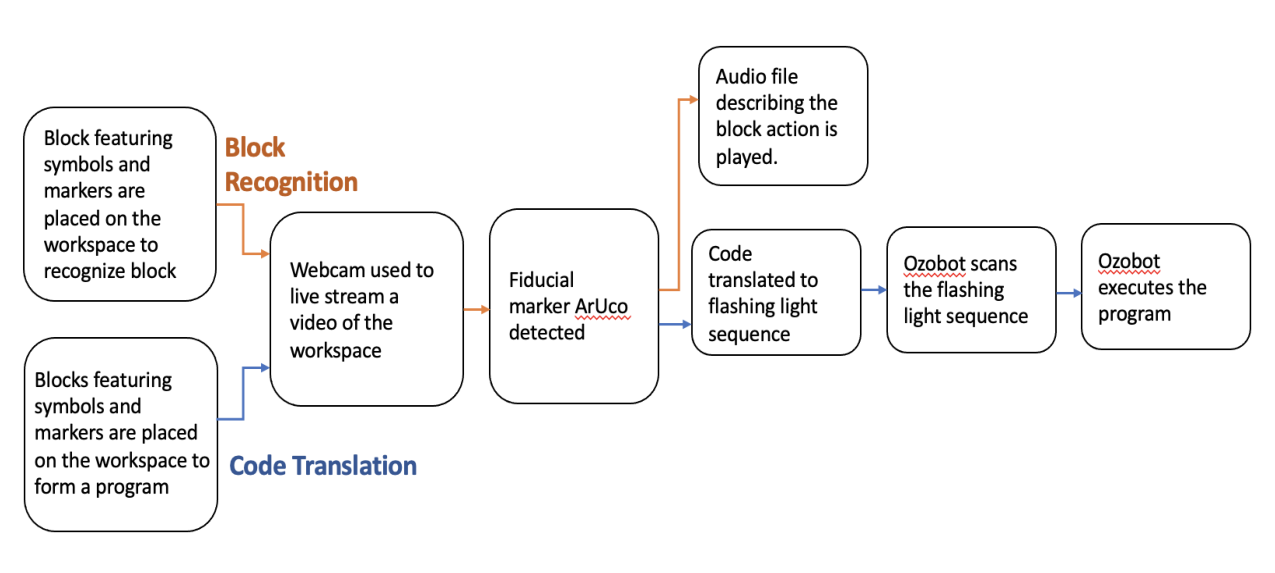
\includegraphics[width=0.9\textwidth]{flowchart.eps}
    \caption{Flowchart of the architecture of my system}
    \label{fig-flowchart}
\end{figure}
\FloatBarrier
In the following section, I analyze the architecture in further detail, for the two main aspects to my system, physical and technical.
\section{Physical Implementation}
In this section, I will present the final physical implementation of my system, after my iterative design process discussed in chapter 4. It consists of wooden blocks that can be put together, a webcam and a workspace set up to detect the wooden blocks.
\subsection{Blocks}
The wooden blocks are the main component of my system. They introduce a tangible alternative to the OzoBlockly platform, and are accessible to all visual abilities.
\subsubsection{Material}
The blocks are constructed from 6mm thick pieces of plywood. Plywood was chosen over acrylic and other plastic materials as it is more robust than acrylic and can be easily recycled. Furthermore, as plywood is easier to paint, I have chosen it over other alternatives to create a high colour contrast on the blocks to make them accessible to children with low vision.
\subsubsection{Shape}
The shape of the blocks is based on the design requirements established in chapter 4. The blocks are a rectangular shape with rounded edges, for safety reasons. A sharp 90 degrees edge was deemed sharp when laser cut in wood, and could potentially injure the user when handling the blocks, especially young children. The shape was designed to be as simple as possible to avoid confusion for visually impaired students when they explore the blocks by tact, as they are already familiar with rectangular shapes. The blocks are a medium size (10cm wide and 5cm high), to facilitate easy interaction with the blocks, however, I also ensured that the pieces are not too large, to develop fine motor skills in younger students. The wooden pieces also feature a distinctive tactile feature on one of the block’s corners, using adhesive Bump-Dots. The round bubble is positioned on the top left hand corner of the blocks to indicate the correct orientation and the user is informed that the bubble indicates the top edge of the block. Additionally, the blocks include magnets situated at the top and bottom edge to help the children clip the blocks together.

\subsubsection{Design}
The wooden blocks feature a tactile symbol and an ArUco Tag, to provide information about the action blocks. The tactile icon is utilised by the user to determine the meaning of the block tactually or by sight, and the ArUCo marker is used for block detection purposes. 
\subsubsection{Tactile Symbol}
Each block features a different tactile symbol that conveys the action meaning and they are placed on the left hand side of the blocks. The tactile icons have been developed using the information acquired during my interview with the QTVI and SEN with minor improvements after the design workshop. The symbols include direction symbols, which are indicated by different arrows, loop symbols, start and end symbols, and variable symbols. The variable symbols differ from the rest, as they feature dots instead of icons, to invite the user to count.  All blocks are accessible to mixed visual abilities as they do not feature braille and only rely on recognition by touch or sight.

\subsubsection{AruCo Marker}
Each block features a unique Aruco marker with varying IDs to enable the detection of the action blocks by the webcam and the system. The markers are placed on top of the blocks on the left hand side. The tags are 3x3 cm to ensure they are big enough to properly be detected by the camera, but also allow enough space for the tactile icon to be placed on the blocks.
\subsubsection{Block Types}
In this section, I will define the different types of action blocks that I have designed for my system. These blocks represent actions that will be executed by the Ozobot.
\subsubsection{Start Block}
\FloatBarrier
\begin{figure}[h]
    \centering
    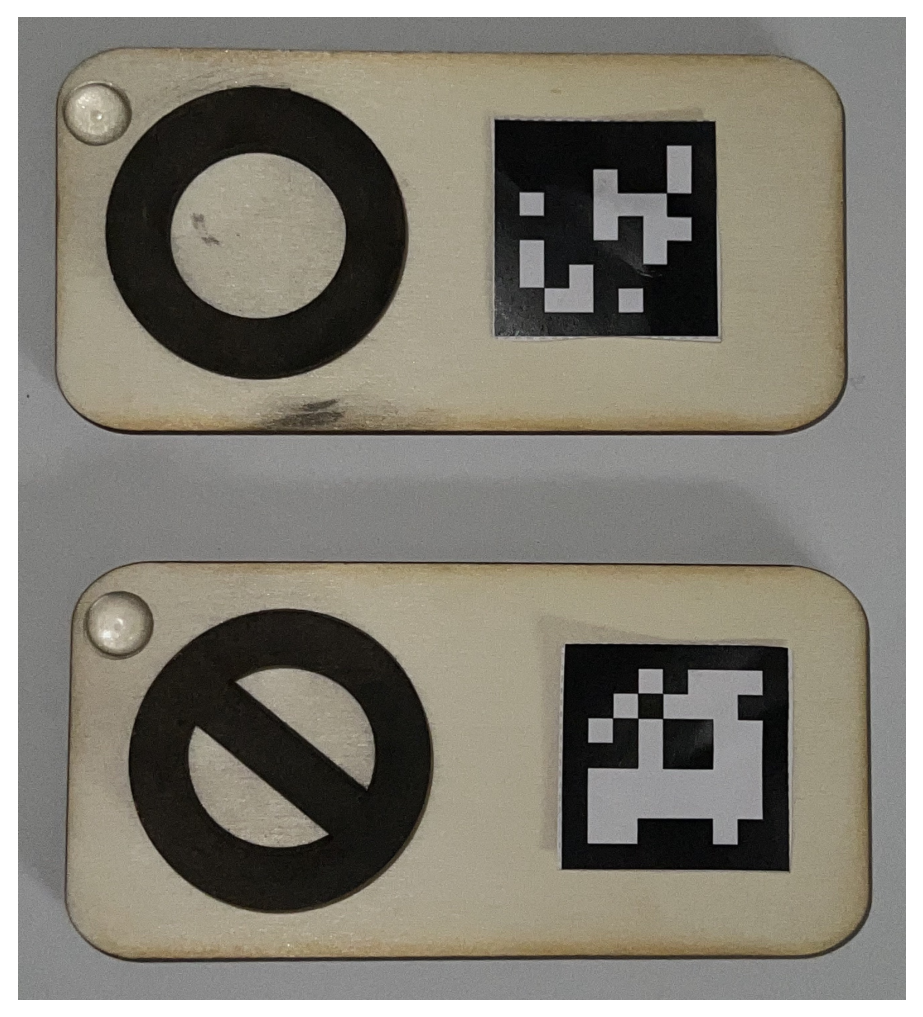
\includegraphics[width=0.3\textwidth]{thesis/startandend.eps}
    \caption{Final Design, at the top: Start Block, at the bottom: End Block}
    \label{fig-startandend}
\end{figure}
\FloatBarrier
The start block features a design that was influenced by my discussions with the experts and favoured by the participants in the design workshop, as the circle relates to the road sign Go and can be matched to the end block block described below. The top block on figure \ref{fig-startandend} represents the embossed circle with a 6mm thickness to allow for easy recognition for visually impaired. 

\subsubsection{End Block}
The end block was designed to relate to the start block, as both the teachers and the participants paired the shape of the start icon to the end icon. For this reason, the end block features a protruding circle with a line through the centre to indicate the "not" sign as shown on figure \ref{fig-startandend}

\subsubsection{Go Forward Block}
\FloatBarrier
\begin{figure}[h]
    \centering
    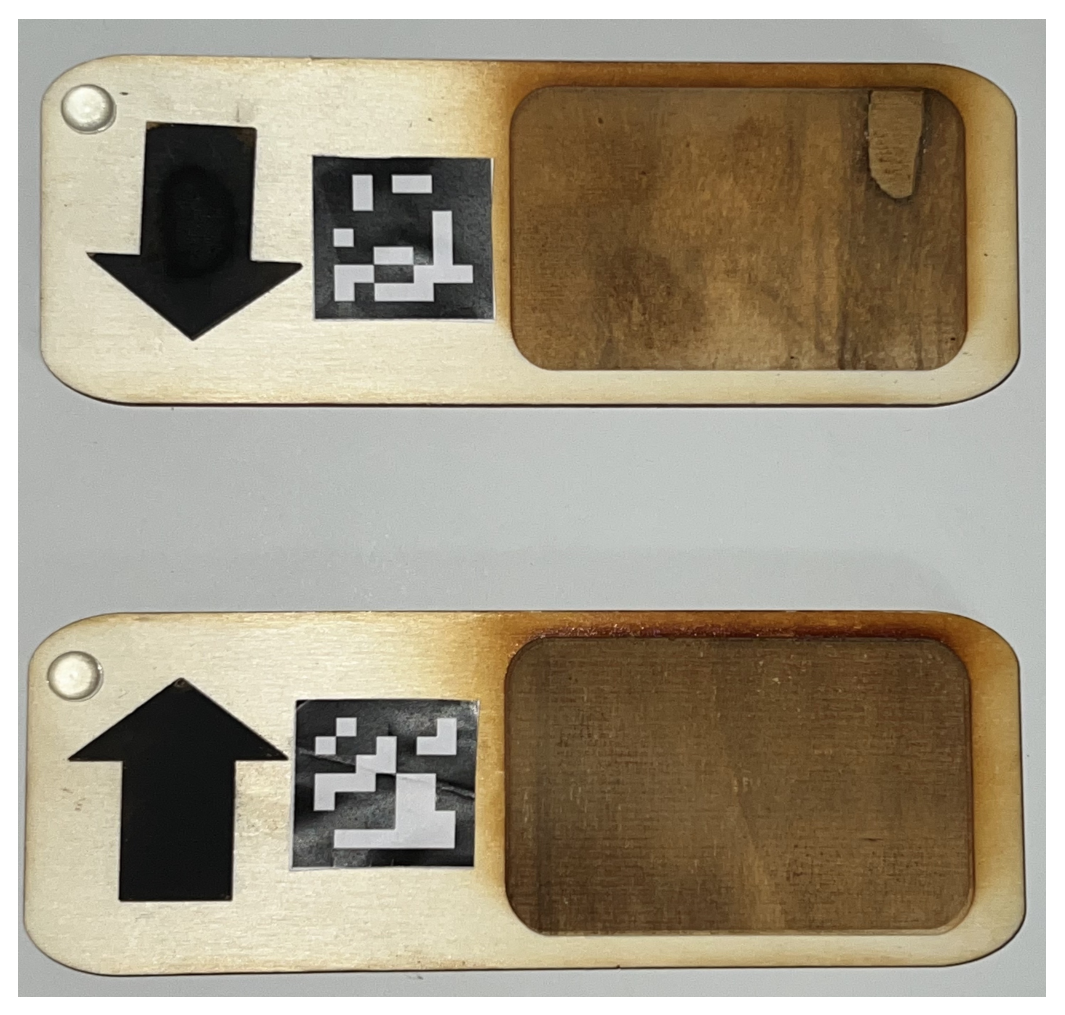
\includegraphics[width=0.3\textwidth]{thesis/backandforth.eps}
    \caption{Final Design, at the top: Go Backwards  Block, at the bottom: Go Forward Block}
    \label{fig-gobackandforth}
\end{figure}
\FloatBarrier
The Go Forward block is a function block. Unlike other blocks, it is 5cm wider to allow for a space to slot the variable blocks. The extra space is engraved around 5mm deep to enable the user to place the smaller variable blocks as seen in figure \ref{fig-gobackandforth}. The slotted variable block indicates the number of steps the robot should move forward. The Go Forward Block features an arrow pointing ahead to depict the action of the robot moving forward and a marker. The arrow design was unanimously favoured by participants and approved by the QTVI and the SEN as a suitable symbol for visually impaired students. 

\subsubsection{Go Backwards Block}
The Go Backwards block is designed similarly to the Go Forward symbol, with an engraved area for variable blocks. It features an arrow pointing downwards and the corresponding aruco tag, as seen on figure \ref{fig-gobackandforth}.

\subsubsection{Turn Left Block}
\FloatBarrier
\begin{figure}[h]
    \centering
    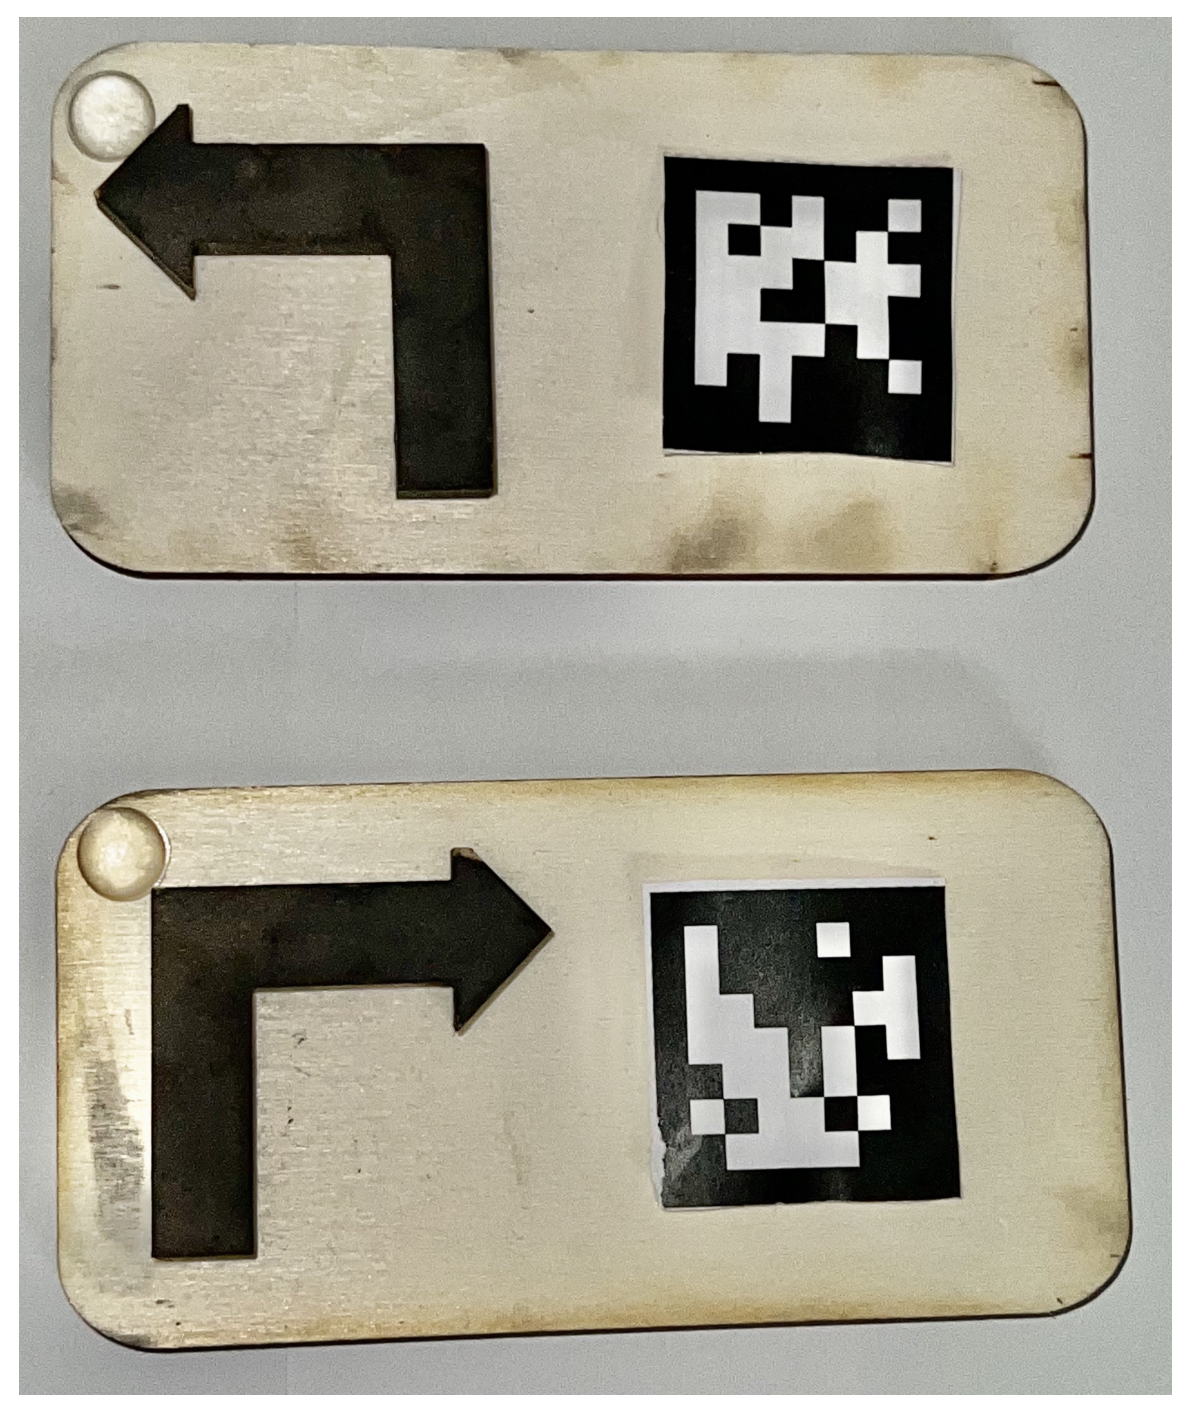
\includegraphics[width=0.3\textwidth]{thesis/leftright.eps}
    \caption{Final Design, at the top: Turn Left Block, at the bottom: Turn Right Block}
    \label{fig-leftright}
\end{figure}
\FloatBarrier
The Turn Left block represents the action of the Ozobot turning 90 degrees to the left, by an arrow that starts with a straight line and then takes a sharp 90 degrees left turn. This design was clear to all participants and deemed simple enough to be understood by students with mixed visual abilities by the expert interviewees.

\subsubsection{Turn Right Block}
The Turn Right Block \ref{fig-leftright} is similar to the previous block, and includes an arrow that begins with a straight line that take a sharp 90 degree turn to the right.

\subsubsection{U-turn to the Right Block}
\FloatBarrier
\begin{figure}[h]
    \centering
    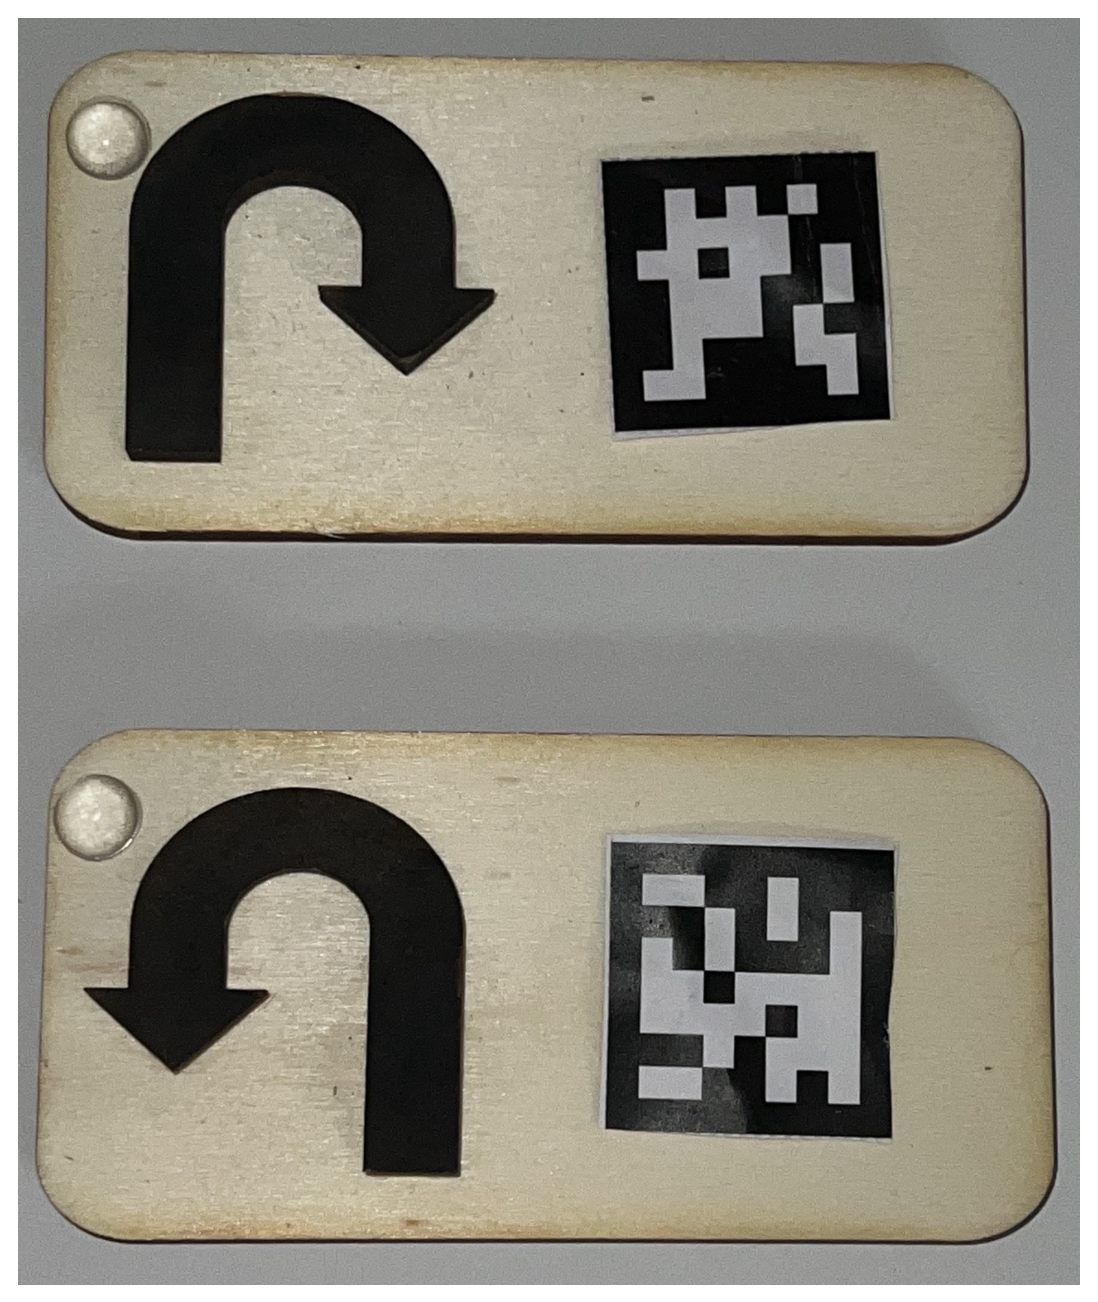
\includegraphics[width=0.3\textwidth]{thesis/tuurn.eps}
    \caption{Final Design, at the top: U-turn to the Right Block, at the bottom: U-turn to the Left Block}
    \label{fig-alluturns}
\end{figure}
\FloatBarrier
The U-Turn to the Right Block features an arrow that begins by a straight line and then curves to the right in a semi-circle with a straight arrow pointing ahead at the end. This design was favoured by the study  participants as 'the curve before the arrow conveys the meaning of fully turning' and it also resembles the u-turn road sign.
\subsubsection{U-turn to the Left Block}
This block is identical to the previous block, but the arrow is pointing in the parallel direction, to the left as shown on \ref{fig-alluturns}

\subsubsection{Start-Loop Block}
\FloatBarrier
\begin{figure}[h]
    \centering
    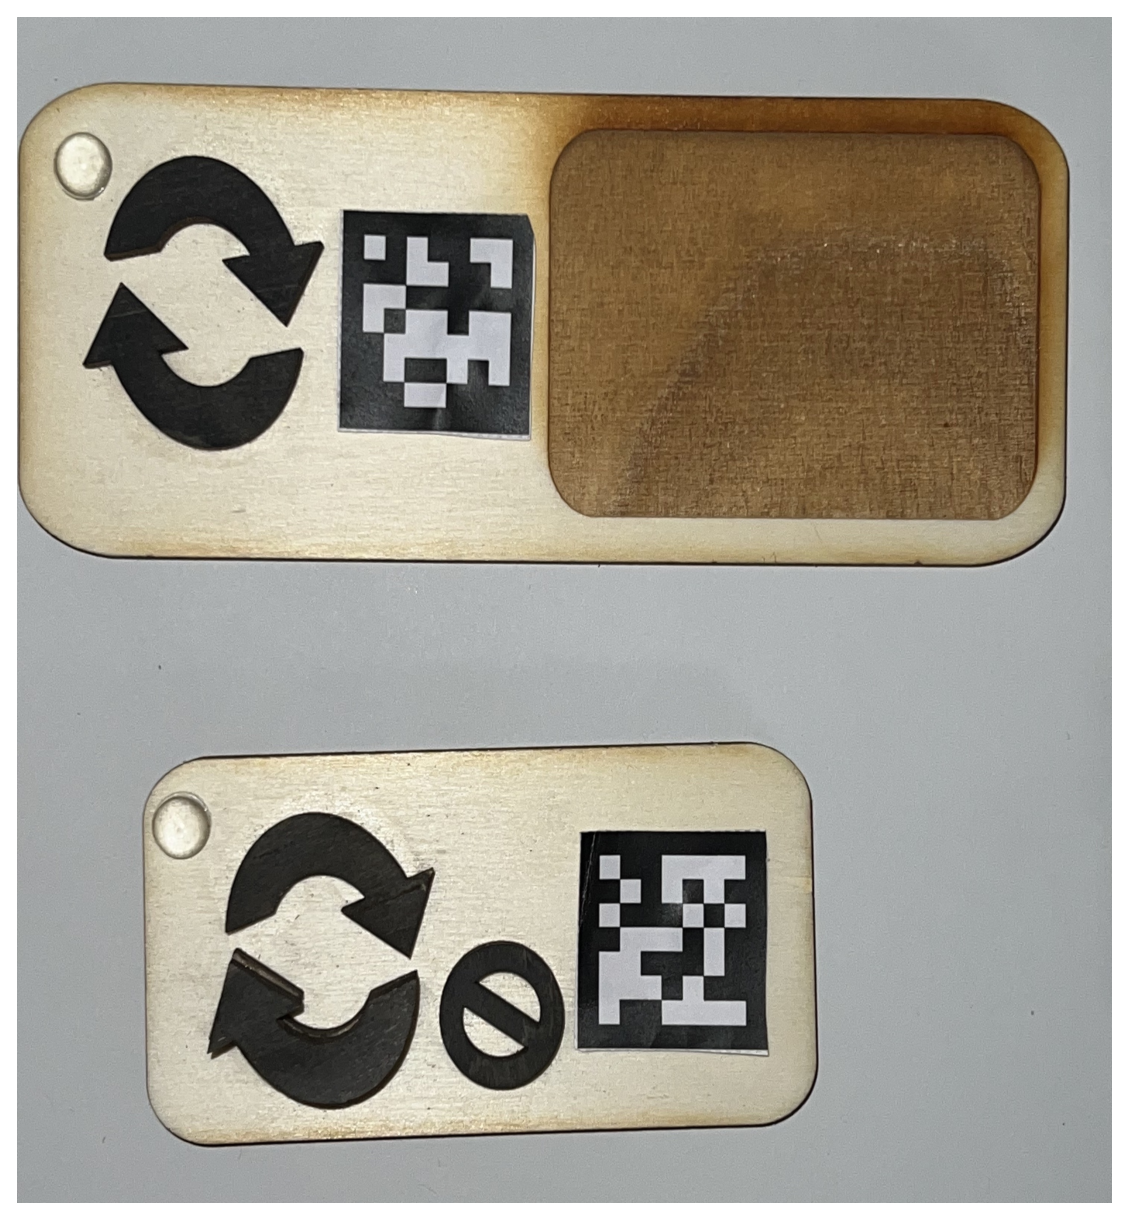
\includegraphics[width=0.3\textwidth]{thesis/startandendloop.eps}
    \caption{Final Design, at the top: Start-Loop Block, at the bottom: End-Loop Block}
    \label{fig-startandendloop}
\end{figure}
\FloatBarrier
The start loop block is a function block with an engraved slot to fit the variable blocks. Similarly to the start and end blocks, participants related the meaning of the start-loop to the end-loop, thus the designs are matched. This also ensures that the children don't have to memorise too many icons. The symbol features two curved arrows pointing to each other in a circular shape. The design was agreed on with the study group as it was the easiest to interpret, since the double arrows convey the meaning of a 'repeat' action. It's also unambiguous and won't be confused with other arrow signs used for directions. The number of loop repetitions is determined by the variable blocks inserted into the slot. Unlike the go forward/backwards blocks, the maximum number of repetitions for the loop block has been set to three. Thus, if the user inserts any variable bigger than three, the system will return an error.

\subsubsection{End-Loop Block}
The end-loop block relates to the start-loop block, it features the same two curved arrows from the previous blocks, with the addition of the 'No' symbol in a smaller size placed to the right of it. The stop icon was made smaller to avoid confusion between the end-loop and End Program blocks. The design was chosen during the design study over other alternatives, as one participant suggested that the End-loop block should feature the icon from the End Program block to match the same pattern and transfer the same meaning of stopping. 

\subsubsection{Variable Blocks}
\FloatBarrier
\begin{figure}[h]
    \centering
    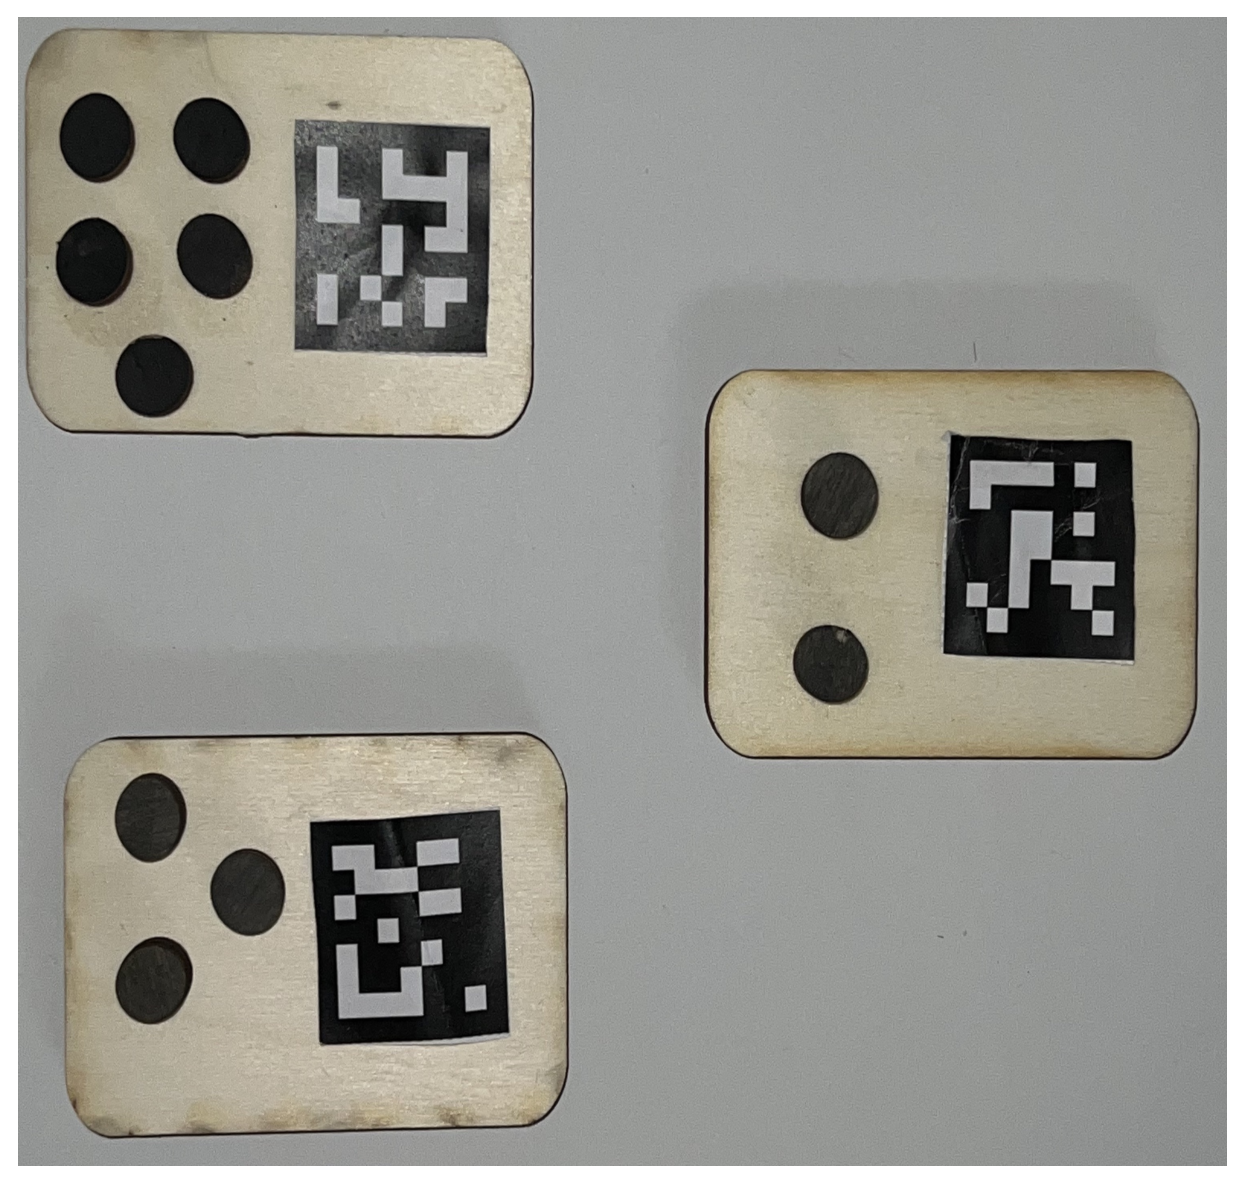
\includegraphics[width=0.3\textwidth]{thesis/finalvariable.eps}
    \caption{Final Design of Variable Blocks}
    \label{fig-variables}
\end{figure}
\FloatBarrier
The variable blocks are smaller sized blocks that are inserted into the function blocks. They determine the input of the Go Forward/Backwards blocks as the number of steps and the input of loops as the number of repetitions. The blocks' design includes a set of dots that are all spaced with a minimum of 6mm to allow for optimal haptic detection, which helps the user count. To maintain consistency with other icons, the dots are circular shapes laser cut from 6mm thick plywood. Bumpons are also not included in the design of the variable blocks, to avoid confusion between the dots and the bumpons when counting. Additionally, the orientation of these blocks is not important as they can be recognised by the system in any orientation. There are three types of variable blocks, as shown in the figures. The decision to have a maximum of five dots was to ensure that my blocks are not too large due to the 6mm gap rule, and due to the fact that visually impaired young children may struggle to count to higher numbers, according to the QTVI. The presence of variable blocks that are fitted into function blocks introduces the computational concept of functions and their input to students. 

\subsection{Workspace}
The workspace is the area where children construct their code sequences. It also has a webcam mounted on a tripod that transfers the code sequence to the system, which then converts it into actions for the Ozobot to perform. I'll describe the different aspects of my workspace in this section.
\subsubsection{Outline}
I elected to outline my system with LEGO bricks rather than trays due to the fact that trays can be too small to fit all the blocks or too high on the edges obstructing the webcam's vision. Furthermore, by using LEGO as outline, the workspace size can be customised. For example, if a larger workspace is required to accommodate more blocks, the user can simply add more bricks to expand the work area. Additionally, using LEGO bricks to define the workplace is a fun and colourful method to do so. Low vision kids may be able to identify
the LEGO's bright colours, and visually challenged students would be able to recognise the outline due to the indents on the LEGO's. Furthermore, they are inexpensive and widely available in most primary schools.

\subsubsection{Surface}
For surface of the workplace, I opted to use non-slip Dycem material [ref] as it stops objects placed on top of it from shifting. Furthermore, it is frequently sold in rolls of two metres or more, allowing it to be cut to fit the surface as needed, and it is available in a range of vibrant colours that low vision pupils can recognise. It is widely used with visually impaired students, as discussed with the teachers in previous sections, so it should be readily available in some schools. It's also inexpensive and robust. I haven't been able to test the dycem material with my system, as it wasn't readily available for me. However, it can be easily incorporated in my system. The teacher simply has to fit the material in the workspace area, outline it with LEGO, and the children can place blocks on top of it. 
\subsubsection{Map}
The workspace also features a map, that is outside of the outlined programming area. It represents the output area of the code constructed in the workspace. 
The map is drawn on A3 paper and is customised for each task. It shows the robot's expected path; the teacher or teaching assistant can set the path by drawing it with a marker and placing a set of blocks at the destination, which the robot will knock down. After the children have been given a description of the route and the task at hand, they clip together the blocks that they believe will allow the robot to reach its destination from its starting position. When the children are done programming, the system scans the blocks and the action is transferred to the Ozobot as a flashing light sequence. The robot then executes the dictated set of actions and if successful at reaching the destination, the set of blocks is toppled by the robot, outputting a sound effect for visually impaired students to recognise that they succeeded. 

\section{Technical Implementation}
The technical design of my system converts the programming blocks scanned by the webcam to a flashing light sequence, used to transmit instructions to the Ozobot or alternatively performs block recognition by reading out the actions displayed on the blocks. The different components interact with each other to program the Ozobot through five main steps: live stream video of blocks, detection of markers, ordering of marker ID, translation to Ozopy, and output light sequence. On the other hand, for block recognition, the components interact differently and fewer steps are required. In this section, I will discuss in more detail each of these steps and their technical aspects. 
 
\subsection{GUI design} 
 
The GUI is designed in a way that when the system starts, the user is presented with two buttons, Translate to Ozopy and Recognise Block. The translate button captures the blocks on the workspace using the webcam and translates it to the Ozopy language, and the ‘Recognise block’ button plays an audio file. When clicked on, both buttons display a window which shows the live streamed video from the webcam.  
I have chosen to implement a GUI framework because it is a very intuitive platform and does not require the use of the terminal or command line. Since this system is primarly designed for teachers and students, I ensured that it is very straightforward to use. It also outputs separate windows depending on the button clicked, this feature avoids any confusion due to clustering of windows when using the system.  
(picture of system)
\FloatBarrier
\begin{figure}[h]
    \centering
    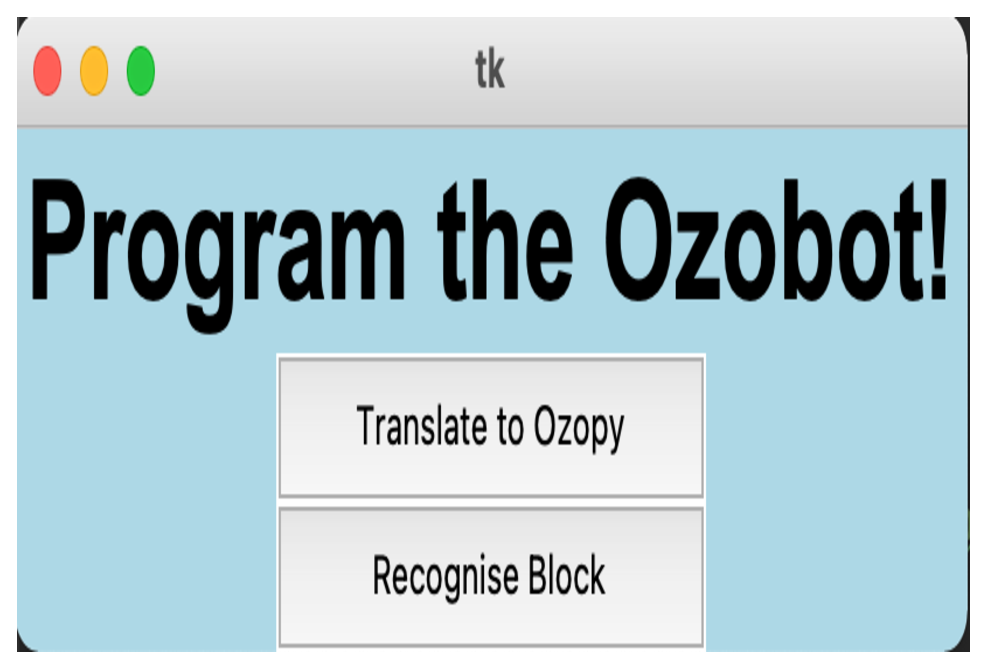
\includegraphics[width=0.5\textwidth]{thesis/gui.eps}
    \caption{GUI Main Window}
    \label{fig-gui}
\end{figure}
\FloatBarrier
\subsection{Detection} 
\FloatBarrier
\begin{figure}[h]
    \centering
    \includegraphics[width=0.5\textwidth]{thesis/detection.eps}
    \caption{Detection of ArUco Markers in my system}
    \label{fig-detection}
\end{figure}
\FloatBarrier
Right before the detection stage, the program loops over the frames of the live streamed video and reads in the images using the imutils library previously mentionned. The detection stage is where the rendered frames are analysed using the OpenCV aruco module and the detectmarker() function described in chapter . 
The detection process outputs a list of markers and their corresponding IDs. 
After the detection process, the IDs are utilised to either identify a block or translate instructions for the Ozobot. 
 
\subsection{Block Recognition}
 
This process involves using the detected marker from the live streamed video to look up prewritten lines of code matching the marker ID to an audio file and finally playing the audio describing the block action. Table \ref{tab-sound} shows an example of this feature.

\subsection{Ordering} 
 
After the blocks are detected and their marker IDs stored in a list, the system orders the marker IDs based on their distance from the start block. This is to ensure the output program is formed in the right order. The system calculates the (x,y) coordinates of the center of the Start block and for every marker in the code sequence using the marker's four detected corners from the detection algorithm. After obtaining the coordinates of all the centers, the coordinates are stored in a list and sorted incrementally compared to the center of the start block. 
The system checks that the first and last marker IDs in the list correspond to the Start blocks and End Program Blocks, respectively. If not, the GUI outputs an error message to notify the user of the issue. This alert is outputted as an audio file, to make the debugging of the program accessible to all visual abilities.  

 
\subsection{Translation to Ozopy}
 
In this stage, the list of marker IDs is translated to code used by the Ozopy language compiler. My system iterates through the ordered marker ID list to look up pre-written lines of code. Each ID has been matched to describe a command. When this ID is identified in the list, its corresponding command is written to a text file called code.ozopy.  
When the system detects a Start-Loop block marker ID, the commands coming after the loop are indented inside the text file. When the End-Loop block is detected, that indentation is decreased. The loop is created using the while command and a variable is initialized and incremented to track the number of iterations. The program is terminated when the End Program marker ID is translated to the ‘terminate(OFF)’ function. This command switches the Ozobot off. 
The lines of commands written to code.ozopy are then ready to be turned to a flashing light sequence. 
 
\subsection{Output}  
This is the last step in the ‘Translate to Ozopy’ workflow. This stage uses the Ozopy language library to turn the list of commands to a light sequence. The library is run using the command ozopython.run and the file name containing the commands, code.ozopy. The ozopython library reads in the lines in the file and converts them to bytecodes. The bytecodes are then converted to color codes and a small window appears on the screen. The window features a white background that allows calibration of the Ozobot, and a load button which plays the sequence of flashing lights. The Ozobot is placed on the screen, with the base of the robot where the sensors reside, facing the load window. It takes in the sequence of colors and then performs the scanned actions when its 'ON' button is pressed.

\subsubsection{Summary}
In this chapter, I have described my final design implementations, both physical and technical. In the following chapter, I will discuss the post prototype user testing I conducted to evaluate the usability of my system.


% -----------------------------------------------------------------------------
\chapter{Post Prototype User Testing}
\label{chap:testing}

After creating a final prototype of my system, I conducted user testing to gather feedback on the design and evaluate the system's usability. The evaluation required participants to complete three short tasks by creating a program that would enable the Ozobot to complete a route drawn on the system's map. Participants were then asked to complete a questionnaire about their experience using the system. The tasks were recorded to later analyse the choices users make while constructing programs and the problems they encountered.

\section{Participants}
Four participants took part in this user study, one of which also participated in the previous design workshop. All participants were chosen as they fit the participation criteria; over 18 years of age, are students, and have little experience with coding. Two of these participants were female while the remaining two were male. No participants had a disability or impairment. All participants were recruited on social media or were contacted after completing the design study. Each participant was given a participation information. If the participant consented to proceed, they were contacted to undertake an in person study and were given a physical consent form once they arrived. 

Recruitment of visually impaired students was attempted on relevant social media groups. I successfully recruited one VI individual, however due to COVID, the participant was unable to complete the study in the required time frame. Testing my system without a key demographic (VI) resulted in the responses to the testing not being as relevant as they possibly could. I attempted to mitigate this limitation through conducting an in-depth co-design process with experts in the field, as described in chapter \ref{chap:design}. In chapter \ref{chap:conclusion}, I will discuss how future work can further refine the design by testing the system with all end-users, including students with visual impairments. 

\section{Testing Procedure}

Each participant completed the study alone or within a pair. P1 and P2 performed the tasks alone while P3 and P4 were paired together. This was a deliberate decision to test if my system accomplishes two main aims: supporting independent use as well as collaborative learning. 

The first part of the study involved describing the aim of the user testing to the participants. The participants were then shown the system and its different components and explained the different actions that the Ozobot can do. I also described the outlined Lego workspace and its purpose, as well as the fact that it can be customised in size and that extra bricks are available if the workspace needed to be expanded. They were then informed that they would need to complete a questionnaire about their experience at the end of the task. I then reminded them that they could withdraw from the study at any point and written consent was obtained at this point.

In the second part of the study, I described the tasks the participants were required to complete and presented the different programming blocks that they can utilise. 

\subsection{Task Design}
The tasks were designed to not only test the usability of my system but also to verify if it fits the low floor, high ceiling, wide walls criteria \cite{CB-lowfloor} described in chapter \ref{chap:context}. Each task aims to introduce a different computational concept, such as loops, sequences, and conditionals, and each task has varying levels of difficulty. The tasks begin with a low threshold to familiarise participants with the system (low floor), then progress to a higher threshold to test if my system is extensive enough to meet the needs of advanced programmers(high ceiling). The chosen questions also have a variety of correct answers, allowing for diverse exploration and encouraging creativity when completing the task (wide walls).

\subsubsection{Task 1}

The first route required the participant to move the Ozobot forward 5cm, turn left 90 degrees and move forward 2cm to finish. This task allows the participant to become familiar with the system and how the start, end and go forward blocks are used, as well as experience using the turn 90 degree blocks and the variable blocks for distance values.
\subsubsection{Task 2}
The second task requires the user to move the Ozobot 5cm forward and then go back to the start position, before completing the second section of the path. This question aims to introduce the concept of conditional statements, even though system doesn't include if else statements, by imposing the condition of completing the first section before being able to move to the second part of the route.
\subsubsection{Task 3}
The final route required the user to follow a 5cm wide square. This task encourages the use of the loop blocks to complete the path, as only two go forward 5cm blocks are available to the participant.
\subsection{Available Blocks}
It was important to limit the number of blocks available to the participants, to ensure they were thinking of the most computationally efficient solutions and not the easiest solutions. 
The following blocks were given to the participants:
\begin{itemize}
    \item  Start Block
    \item End Block
    \item 2 Go Forward Blocks
    \item 2 Go Backward Blocks
    \item 6 Variable Blocks (2x2, 2x3, 2x5)
    \item 2 Turn Left 90 Degrees Blocks
    \item 2 Turn Right 90 Degrees Block
    \item 1 U-Turn Left Block
    \item 1 U-Turn Right 180 Block
    \item 1 Start Loop Block
    \item 1 End Loop Block
\end{itemize}

\subsection{Questionnaire}
After the user testing, participants were sent a Google Forms questionnaire to provide feedback about their experience using the system. The survey is a mixture of scale, multiple choice, and long answer questions to get their opinion on the design and usability of the system as a whole. The questionnaire can be found in appendix A.

\section{Task Results}
\subsection{Prior To The task}

Prior to completing the task, I wanted the participants to get familiar with loading the program on the Ozobot, as this can be a complex process. I didn't want the participants to be frustrated with the loading process during the tasks, as this can break their concentration. Thus, I invited the participants to make a few attempts at loading and running an example program. 

Some issues arose at the beginning of this activity. All participants struggled to correctly load the program onto the Ozobot, even though I demonstrated the process. Firstly, participants couldn't properly calibrate the Ozobot, due to not being able to locate the power button on the side of the Ozobot Bit. They also had to hold down the power button for 2 seconds until the top LED light blinks white, then release the power button to calibrate. Most participants struggled with this and often double clicked or released the button too early. Participants also had to double click the power button to run the program after the Ozobot was loaded. However, some users would double click too slowly, which accidentally turns off the robot, or double click too fast, so the robot only senses one click. Another general comment was that the different button clicks required is confusing. Some participants also found it difficult to differentiate the front of the Ozobot from the back, so that was also explained to them. I offered assistance to the participants after a number of failed attempts at loading the program. All users could successfully load and run the program after a few practice attempts. 

Participants were also given an overview of the GUI's various features and their functions, such as the Block Recognition tool. Before beginning the tasks, P2, P3, and P4 all tried out this function. Most participants tested the functionality with the loop blocks and the start and end blocks, with the general consensus being that the three users understood the icons on the blocks but wanted to double-check that they had correctly interpreted the action on the block. P1, on the other hand, indicated that he did not need to utilise the block recognition tool because he was a participant in the design workshop and knew exactly what each block represented.

\subsection{During The Task}
All four participants completed the three tasks.
\subsubsection{Task 1}
This task was completed with a few issues caused by the participants not understanding the use or orientation of the blocks. However, participant P1, who also took part in the design workshop, completed the task with mostly no difficulty as he had prior knowledge about the system's components.

After being described the task, all participants explored the different blocks and chose the most relevant blocks to start their program: the go forward and turn left block, and the start and end blocks. 
P2, P3 and P4 all wondered about the function of the engraved spot in the Go Forward block. P3 and P4, who were working together, figured out the purpose of the slot, when P3 identified that 'there are some blocks with dots that are the only ones small enough to fit in there'. The pair quickly recognised that the dots were a numeral system. P2 identified the same relationship after I hinted to explore the different sizes of the blocks. All four participants asked about the relationship between the dots and the distances, I explained that one dot represents one step which is 1cm. This suggests that the design might need to be altered to show the true value of distance.
\FloatBarrier
\begin{figure}[h]
    \centering
    \includegraphics[width=0.3\textwidth, height = 5cm]{thesis/task1.eps}
    \caption{Program Created for Task 1}
    \label{fig-task1}
\end{figure}
\FloatBarrier
P3 and P4 also struggled in assembling the program in the correct way, by initially putting the rectangular blocks side by side to construct a horizontal sequence. However, they quickly noticed the magnets on both sides of the blocks and realised the blocks should be placed vertically to clip together. Alongside with P2, all three participants had trouble deciding the correct orientation of the blocks. They identified the presence of the bumpons on the corner of the block, but they were unsure if the bumpons were meant to be in the top left corner or the bottom right corner, if the block is flipped. P3 realised the correct orientation when she noticed that the magnets on the start block are only on one side of the block, suggesting that side corresponds to the bottom of the block, which places the bumpon on the top left hand corner. P2, on the other hand, experimented with both orientations, choosing the wrong orientation first. She then intuitively chose the correct orientation because she assumed the icons should be on the left hand side of the block, as the block would be read left to right. She also identified the magnets when constructing the program, proving her right in the chosen orientation. This suggests that the combination of magnets and bumpons is a good indication of the correct orientation of the blocks. 

Additionally, P3 inquired about the possibility of creating programs upwards, with the start block being closest to the participant. They commented that since the robot's path starts closest to me, so should the program. This question was explored with the other participants, to get their preference. The three other participants felt it was more natural to start the program from the top down, like it currently is. They stated it was easier to read the code downwards. 

Finally, P1 had forgotten to include the end block at the end of the program, resulting in the system playing an error message. The participant immediately rectified his mistake, suggesting that error messages are clear and helpful.

\subsubsection{Task 2}
Participants had less issues when completing task 2, as they were all now familiar with the correct orientation and the different components of the blocks. 

P1 completed the task with no issues.

P3 and P4 first manually moved the robot to complete the 2 sections of the path, suggesting they had to experiment to come up with the algorithm. They came up with one way of completing the route but as they were building their code they realised that they only had 2 forward blocks, when they needed 3. The two participants went back to the route and tried moving the Ozobot with a different method. P3 reminded his partner 'we forgot it can go backwards!', the pair quickly found the answer afterwards. (f b r f)

P2 completed the first section of the path with ease, then struggled to understand the orientation of the robot compared to the orientation of the arrows on the block when completing the second section. She instructed the Ozobot to move forward, do a u-turn and then move forward again. The participant knew she had to use the backwards block to complete the second section, however she had trouble deciding which way to orient the Ozobot first. I suggested that she runs the program manually step by step using the robot. When she put down the robot to follow the path, she did not orient it forwards, which suggests that the design of the robot still causes confusion about its orientation, even after the demonstration in section 7.3.1. The robot's design could be changed to help with this. 

\subsubsection{Task 3}
\FloatBarrier

\begin{figure}[h]
\centering
\begin{subfigure}{.5\textwidth}
  \centering
  \includegraphics[width=0.8\textwidth,height = 7cm]{thesis/square.eps}
  \label{fig-square}
\end{subfigure}%
\begin{subfigure}{.5\textwidth}
  \centering
  \includegraphics[width=0.8\textwidth, height=7cm]{thesis/square2.eps}
 
  \label{fig-square2}
\end{subfigure}
\caption{Programs Created for Task 3}
\label{fig-task3}
\end{figure}
\FloatBarrier
All participants realised this task required the use of a loop due to the constraint on the number of blocks available. The participants inquired if the number of repetitions in the loop was also decided by the numeral blocks used previously. I confirmed their hypothesis. 

P1 effectively selected the start-loop and end-loop blocks and placed them correctly. He then traced the outline of the route on the map with his finger, reading out the required instructions at each section, to finally successfully build the program.

P3 and P4 conducted manual testing with the robot again, to aid with constructing the code. They successfully identified the need to use the loop function to complete the task and placed the start-loop and end-loop blocks within the workspace. They identified the repeated pattern of going forward and turning to complete a square, and divided the program into sections to count the number of repeats they would use. 
P2 also successfully completed the task using a similar approach to P3 and P4. She however wrote down the different instructions and directions before coding the program, to ensure her reasoning was correct.


\section{Questionnaire Results}
The results of the survey are detailed in appendix \ref{appx:survey}. In this section, I will discuss the main insights gathered from the responses to the feedback questionnaire. To analyse the survey data, the distribution of the observations was generated and graphed in a bar chart, and the mean of the linear scale answers was calculated.

\subsubsection{Question: What do you think of the symbols used for the blocks? Any comments?}
The first section of this question featured a linear scale from 1 to 5, to allow the user to choose a value between clear and confusing. All participants rated the action symbols close to clear, with a response mean of 1.5.
There was a long answer text for the 'Any comments?' section of the question, to gather additional individual feedback. 
Two of the participants stated that the icons clearly indicated which action they were representing, and the 'recognise block' feature made the few symbols they were uncertain about, clear. Two participants raised the issue that they questioned the values of the variable blocks and the distance they represented. One participant additionally commented that the joint meaning of the variables for distances and number of iterations, can be confusing. He suggested that the distance metrics and the number of loops be distinguished by different variable blocks. This suggests that the real-world distance should be explicitly depicted in the design, as well as a clear design distinction between the various uses of variables.


\subsubsection{Question: What would you improve about the design of the blocks?}
This was a long answer question, to get feedback about the overall design of the blocks.
Two participants mentioned that the design of the blocks was engaging and easy to understand, commenting that the color contrast and the icons made it easy to understand the actions depicted. Three participants stated that they would have liked if the correct orientation of the blocks was clearer from the start. One participant suggested replacing the bumpon with a drawn arrow pointing the right orientation. 

\subsubsection{Question: How did you find the process of assembling code? Why?}
This question was structured similarly to question 1 and featured a linear scale for the user to pick a value between difficult and easy and a text input for the reasoning behind the answer. Participants rated their code assembly experience with an overall mean of 1.75.

P1 and P3 commented that the magnets were very useful in assembling the code and putting the blocks together, however P3 also stated that their experience started off fairly confusing as they were not able to determine the correct orientation of the block. P2 and P4 had similar feedback, struggling to determine the correct orientation of the blocks at first.  All participants reported that the code assembly was much easier after they were familiar with the right block orientation. The answers to this question and the previous one suggest that the correct way of assembling blocks should be explained prior to using the system.

\subsubsection{Question: How did you find the tasks you were set to complete? What difficulties have you encountered?}
The tasks were rated as close to easy by all participants, with a mean of 1.5. 

P1 and P2 remarked that constructing the solution out of the limited pieces supplied was the difficult part, with both participants admitting that it pushed him to think of more creative solutions. The exercises were deemed rather easy by all participants, after they understood how to arrange the blocks and which way they fit together. This shows that the orientation of the blocks may become a burden during learning, and that the user may prefer a design that expresses the orientation more explicitly or does not require it. 


\subsubsection{Question: How would you rate the workspace? Why?}
All participants rated the workspace as creative. The general feedback was that participants enjoyed building programs in a specific area. P3 and P4 participants remarked that having an outline space made it feel like they were working in a defined programming environment, and that they enjoyed customising the size of the workspace by adding or removing Lego. One participant noted that it might be more convenient to have an outline that is bound together, so the outline doesn't break. They reported that while building programs, they sometimes accidentally hit the Lego with their hand which caused the outline to shift. 

\subsubsection{Question: How did you find the 'Recognise Block' feature? Why?}
All participants rated the block recognition close to helpful, with a mean response of 1.25. The general consensus was that participants appreciated having a feature in the GUI that confirmed the actions of the blocks, before they started assembling code. One participant suggested adding a feature in the block recognition that also tells the user if the block is placed in the right orientation, so that users don't struggle initially.


\subsubsection{Question: In what setting would you use this system and why?}
This is a multiple-choice question with the following options: Pair, Alone, or Group, to determine which method of interaction is preferred. 
The majority of participants preferred to use the system alone or in pairs. P3 and P4 both stated that working on the tasks with a partner was enjoyable because they could discuss solutions with one another. This reaction shows that my system would be best employed in a group setting and that it effectively encourages collaborative learning, something students with visual impairments typically miss out on due to the assistance bubble effect.

\subsubsection{Question: How would you rate your overall experience? Justify your answer.}
All participants rated their experience with the system as enjoyable, with a mean of 1.25.
P3 and P4 stated that it was fun to work together and that they enjoyed the problem solving process. P1 and P2 also described the experience as fun and engaging, but they both raised the issue with the process of loading programs, stating that it was often frustrating and time consuming. 

\subsubsection{Question: Any comments or suggestions for the overall system?}
All participants stated that the process of loading the code and running it with the Ozobot is confusing and time consuming. Most participants felt they needed assistance loading programs onto the Ozobot at some point during the tasks, even after the demonstration. One participant said they couldn't find the Ozobot's power button and had forgotten how many button pushes were required for each operation. Two additional participants claimed that when completing the activities, they were unsure about the robot's orientation, which caused them to make mistakes in code assembly. This implies that improving the robot's design to make it more clear and user-friendly would improve the user experience. 

One participant suggested turning the system to a mobile application, as that would make the system more lightweight and easier to scan the blocks with, rather than needing a whole setup, with a webcam and tripod.

\subsection{Discussion of questionnaire results}
To summarise, the survey results provided me the insight I needed to evaluate my system and identify critical areas where it might be improved.

All participants reported that they enjoyed using the system and completing the tasks.  The design of the blocks also received a lot of great feedback, with participants reporting that they were simple to use and understand, suggesting that the iterative design process was successful. one of the principal design goals of the system. 

However, some areas of improvement were identified by participants.
Firstly, most participants had difficulty determining the correct orientation of the blocks at first glance, but after inspecting them and discovering the magnets and bumpons, they correctly positioned the blocks. This suggests that some time should be allocated for users to explore the different blocks, before starting activities. Additionally, when dealing with children, it would be ideal for the teacher to state the correct orientation beforehand. In the case of VI children, the bumpons are a clear indicator for block orientation according to the SNE, so this should not be an issue if my prototype were to be tested with VI individuals.

Second, the majority of participants said that loading programs was difficult and took several attempts. There is no way to rectify this as the method used to load the program is part of the design of the Ozobot itself, not my system. Alternative robots could be explored to be used with my system.
Finally, one user suggested that the system be made 'more flexible' by developing an app. Their main suggestion was to let the user take a picture of the blocks once they are done assembling the code, and upload it to the system to translate it to code. An app would increase the system's adaptability and eliminate the need for the user to have a specialised setup. My system could easily be translated to a mobile platform as the marker detection algorithm is also compatible with smartphones. 

Overall, I have created a system built that has been deemed to be engaging and and fun, while supporting the learning of basic concepts of computing, such as sequences, loops and termination.


% -----------------------------------------------------------------------------

\chapter{Conclusion and Further Work}
\label{chap:conclusion}

\noindent
\section{Overview}
During this project, I have created an accessible programming platform for the Ozobot, to make programming robots accessible to mixed visual abilities. The system is a tangible user interface, composed of tangible programming blocks, the Ozobot and a workspace for young students to assemble programs in the physical world. It allows the introduction of computational thinking to young students by teaching them concepts such as loops, sequences and functions.


While completing the project, I first set out to research current systems used to teach computational thinking to children as well as tools used by those with a visual impairment to learn how to program, documented in \ref{chap:context}. Many of the explored accessible systems required proficiency using accessibility software, such as screen readers, and involved complex syntax, making them unsuitable for younger students. Other commercially available TUIs that relate to my system such as Torino and Osmo were also explored. However, these systems were often very expensive due to the custom electronics featured within the device and unsuitable for use within the classroom. This initial research emphasised the importance of creating a low-cost and accessible programming system for younger students.

The second step of my project was to research tactile devices available for the classroom and personal use and formulate methods in which these systems could be adapted to make them accessible to those with visual impairment. One such device, known as Osmo, is an app for the iPad that captures physical code blocks placed on the work surface and displays the result of the program on the screen. Many of the other devices are similar to Osmo but feature varying output methods, including allowing control of a robot. The primary issue with using these systems to teach programming to children with a visual impairment is that the blocks only feature visual information. Adapting these blocks to feature Braille or protruding icons would allow these systems to be more accessible, the latter of which I chose to investigate further. The robot I chose to utilise throughout this project is the Ozobot, as it is relatively inexpensive and small enough to be used on tabletops.
Thirdly, I performed a user design study which assisted me in creating a tactile icon system for the faces of the puzzle pieces that is universally understood. The study involved participants modelling or describing tactile symbols to represent actions the Ozobot, a desktop robot, could perform. The results suggested that the shape and the orientation of the icon are the favoured features of a symbol to represent information. The preferred shape used throughout was an arrow that featured bends or loops to represent the actions; move, turn and loop. In addition to this, the study revealed that the proposed design of the puzzle blocks was believed to be sufficient enough to represent the orientation of the pieces.
The fourth step of my project was to design the physical puzzle pieces and create the tactile icons that featured on the surface. I chose to design the puzzle pieces similar to the block design of visual languages, such as Scratch and OzoBlockly. This design choice allows the student to transfer any existing knowledge of these programming IDEs onto the system I have designed. Using the information gained from the user design study, I decided to create the icon designs utilising mostly arrows and related symbols seen in everyday life, such as the u-turn sign, the go sign and the ”do not” symbol. I chose to engrave lines onto the surface of the arrows to represent numerical values as this made the blocks more robust than having them protruding and each line could still be determined clearly. The one exception to this rule was the loop block, as I found fitting the lines onto the symbol difficult as the arrowhead was too small.
The fifth step of this project was to develop a technical system that could effectively detect these blocks when placed on a surface. The GUI features a webcam display window and two buttons that allow for the preview image or an alternative image from file to be used for translation. The main feature of this system is the AprilTag detection algorithm. An AprilTag marker is present on each block, which allows for efficient and robust detection methods to be used instead of a custom shape detector. The blocks are ordered by the system by their distance from the start marker and the program checked to ensure it satisfies all validity requirements. For example, the program is checked to ensure one end loop block is present for every start loop block. The actions detected by the system are then converted to a flashing light sequence using the OzoPython language and can then be loaded onto the Ozobot. The OzoPython language provides functions for basic movements the Ozobot can perform, such as move forward or turn, and converts these to the light sequence bytecodes required.
The final step of this project, after creating the prototype, was to perform a post-prototype study to analyse the system’s effectiveness and ease of use. The study involved four participants creating code for the Ozobot to complete four different routes. These routes challenged the participant’s resource management and forced them to consider alternative solutions due to the limited number of blocks. The results suggested that the orientation of the blocks was troublesome to gauge from the current design. Therefore alternatives, such as providing a tactile symbol on the top of the block to represent up, need to be further investigated. In addition to this, one participant stated that the number of iterations for the loop block was unclear, due to the nature of the design. They interpreted that the loop symbol itself indicated one iteration and the value to the right represented the number of extra repeats, rather than the total. However, all participants were able to identify all blocks successfully and complete all tasks assigned, suggesting that the design of the icons is effective at portraying the actions but requires adjustments to be effortlessly intuitive. Feedback from the post-activity questionnaires indicated that the system was intuitive to use and effectively assisted users in developing basic programming skills, as many participants had not programmed before this task. The questionnaire supported the issue raised above surrounding the ascertainment of the orientation of the blocks. Many users stated that the orientation of the blocks was confusing, suggesting that an amendment to the design of either the face of the blocks or to the blocks themselves, may aid with the intuitiveness of the design.

\section{Limitations}

\section{Future Work}
\begin{enumerate}
\item (Re)summarise the main contributions and achievements, in essence
      summing up the content.
\item Clearly state the current project status (e.g., ``X is working, Y 
      is not'') and evaluate what has been achieved with respect to the 
      initial aims and objectives (e.g., ``I completed aim X outlined 
      previously, the evidence for this is within Chapter Y'').  There 
      is no problem including aims which were not completed, but it is 
      important to evaluate and/or justify why this is the case.
\item Outline any open problems or future plans.  Rather than treat this
      only as an exercise in what you {\em could} have done given more 
      time, try to focus on any unexplored options or interesting outcomes
      (e.g., ``my experiment for X gave counter-intuitive results, this 
      could be because Y and would form an interesting area for further 
      study'' or ``users found feature Z of my software difficult to use,
      which is obvious in hindsight but not during at design stage; to 
      resolve this, I could clearly apply the technique of Smith [7]'').
\end{enumerate}

% =============================================================================

% Finally, after the main matter, the back matter is specified.  This is
% typically populated with just the bibliography.  LaTeX deals with these
% in one of two ways, namely
%
% - inline, which roughly means the author specifies entries using the 
%   \bibitem macro and typesets them manually, or
% - using BiBTeX, which means entries are contained in a separate file
%   (which is essentially a databased) then inported; this is the 
%   approach used below, with the databased being dissertation.bib.
%
% Either way, the each entry has a key (or identifier) which can be used
% in the main matter to cite it, e.g., \cite{X}, \cite[Chapter 2}{Y}.
%
% We would recommend using BiBTeX, since it guarantees a consistent referencing style 
% and since many sites (such as dblp) provide references in BiBTeX format. 
% However, note that by default, BiBTeX will ignore capital letters in article titles 
% to ensure consistency of style. This can lead to e.g. "NP-completeness" becoming
% "np-completeness". To avoid this, make sure any capital letters you want to preserve
% are enclosed in braces in the .bib, e.g. "{NP}-completeness".

\backmatter

\bibliography{dissertation}

% -----------------------------------------------------------------------------

% The dissertation concludes with a set of (optional) appendicies; these are 
% the same as chapters in a sense, but once signaled as being appendicies via
% the associated macro, LaTeX manages them appropriatly.

\appendix

\chapter{Post Prototype Feedback Survey}
\label{appx:survey}

Content which is not central to, but may enhance the dissertation can be 
included in one or more appendices; examples include, but are not limited
to

\begin{itemize}
\item lengthy mathematical proofs, numerical or graphical results which 
      are summarised in the main body,
\item sample or example calculations, 
      and
\item results of user studies or questionnaires.
\end{itemize}

\noindent
Note that in line with most research conferences, the marking panel is not
obliged to read such appendices. The point of including them is to serve as
an additional reference if and only if the marker needs it in order to check
something in the main text. For example, the marker might check a program listing 
in an appendix if they think the description in the main dissertation is ambiguous.

% =============================================================================

\end{document}
